\RequirePackage{plautopatch}
\documentclass[uplatex, a4paper, 14Q, dvipdfmx]{jsarticle}
\usepackage{docmute}
\usepackage{../mypackage_for_segal}

\title{完備Segal空間}
\author{よの}
\date{\today}

\begin{document}

\maketitle

\begin{abstract}
  新しい無限圏のモデルとして, \cite{Rez00}で完備Segal空間が定義された.
  本稿は\cite{Rez00}のlecture noteである\cite{Ras18}をまとめたものである. 
\end{abstract}

\tableofcontents


\section{単体的空間} \label{sec:simplicial_space}

単体的集合には, 通常の圏の脈体(nerve)と位相空間の特異単体(singular functor)という2つの特別なクラスがある.
高次圏論では, この圏論とホモトピー論を同時に一般化した枠組みで考える必要がある. 
この章では, 2つの単体的集合のクラスを1つにまとめる方法として, 単体的空間を考える. 

\begin{definition}[単体的集合]
  関手$\Delta^\myop \to \Set$を単体的集合(simplicial set)といい, 単体的集合の圏$\Fun(\Delta^\myop,\Set)$を$\sSet$と表す. 
\end{definition}

% 圏の脈体は次のように表せる. 

\begin{definition}[単体的空間]
  関手$\Delta^\myop \to \sSet$を単体的空間(simplicial space)といい, 単体的空間の圏$\Fun(\Delta^\myop,\sSet)$を$\sSpace$と表す. 
\end{definition}

\begin{remark} \label{rem:bisimplicial_set}
  積-Hom随伴より, 次の同型が存在する. 
  \begin{align*}
    \sSpace \cong \Fun(\Delta^\myop,\sSet) \cong \Fun(\Delta^\myop, \Fun(\Delta^\myop,\Set)) \cong \Fun(\Delta^\myop \times \Delta^\myop, \Set)
  \end{align*}
  よって, 単体的空間は両単体的集合(bisimplicial set)とも呼ばれる. 
\end{remark}

\begin{remark} \label{rem:diagram_of_simplicial_space}
  \cref{rem:bisimplicial_set}より, 単体的空間は次のように表せる. 
  ここで, $X_{i,j}$は集合であり, $X_{i,-}$や$X_{-,j}$は単体的集合である. 
  % https://q.uiver.app/#q=WzAsMjQsWzAsMCwiWF97MCwwfSJdLFsxLDAsIlhfezEsMH0iXSxbMCwxLCJYX3swLDF9Il0sWzEsMSwiWF97MSwxfSJdLFswLDIsIlhfezAsMn0iXSxbMSwyLCJYX3sxLDJ9Il0sWzIsMCwiWF97MiwwfSJdLFsyLDEsIlhfezIsMX0iXSxbMiwyLCJYX3syLDJ9Il0sWzMsMCwiXFxjZG90cyJdLFs0LDAsIlhfey0sMH0iXSxbMywxLCJcXGNkb3RzIl0sWzQsMSwiWF97LSwxfSJdLFszLDIsIlxcY2RvdHMiXSxbNCwyLCJYX3stLDJ9Il0sWzAsMywiXFx2ZG90cyJdLFsxLDMsIlxcdmRvdHMiXSxbMiwzLCJcXHZkb3RzIl0sWzAsNCwiWF97MCwxfSJdLFsxLDQsIlhfezEsLX0iXSxbMiw0LCJYX3syLC19Il0sWzQsMywiXFx2ZG90cyJdLFszLDQsIlxcY2RvdHMiXSxbMywzLCJcXGRkb3RzIl0sWzAsMV0sWzEsMCwiIiwyLHsib2Zmc2V0IjoxfV0sWzEsMCwiIiwxLHsib2Zmc2V0IjotMX1dLFswLDJdLFsyLDNdLFsxLDNdLFsyLDAsIiIsMSx7Im9mZnNldCI6MX1dLFsyLDAsIiIsMSx7Im9mZnNldCI6LTF9XSxbMywxLCIiLDEseyJvZmZzZXQiOjF9XSxbMywxLCIiLDEseyJvZmZzZXQiOi0xfV0sWzMsMiwiIiwxLHsib2Zmc2V0IjoxfV0sWzMsMiwiIiwxLHsib2Zmc2V0IjotMX1dLFs0LDJdLFs0LDIsIiIsMSx7Im9mZnNldCI6LTJ9XSxbNSwzXSxbMiw0LCIiLDEseyJvZmZzZXQiOjF9XSxbMiw0LCIiLDEseyJvZmZzZXQiOi0xfV0sWzQsMiwiIiwxLHsib2Zmc2V0IjoyfV0sWzQsNV0sWzUsNCwiIiwxLHsib2Zmc2V0IjotMX1dLFszLDUsIiIsMSx7Im9mZnNldCI6MX1dLFszLDUsIiIsMSx7Im9mZnNldCI6LTF9XSxbNSwzLCIiLDEseyJvZmZzZXQiOjJ9XSxbNSwzLCIiLDEseyJvZmZzZXQiOi0yfV0sWzYsMV0sWzEsNiwiIiwxLHsib2Zmc2V0IjotMX1dLFsxLDYsIiIsMSx7Im9mZnNldCI6MX1dLFs2LDEsIiIsMSx7Im9mZnNldCI6Mn1dLFs2LDEsIiIsMSx7Im9mZnNldCI6LTJ9XSxbNywzXSxbMyw3LCIiLDEseyJvZmZzZXQiOjF9XSxbMyw3LCIiLDEseyJvZmZzZXQiOi0xfV0sWzcsMywiIiwxLHsib2Zmc2V0IjoyfV0sWzcsMywiIiwxLHsib2Zmc2V0IjotMn1dLFs2LDddLFs3LDYsIiIsMSx7Im9mZnNldCI6MX1dLFs3LDYsIiIsMSx7Im9mZnNldCI6LTF9XSxbOCw3XSxbNyw4LCIiLDEseyJvZmZzZXQiOjF9XSxbNyw4LCIiLDEseyJvZmZzZXQiOi0xfV0sWzgsNywiIiwxLHsib2Zmc2V0IjoyfV0sWzgsNywiIiwxLHsib2Zmc2V0IjotMn1dLFs4LDVdLFs1LDgsIiIsMSx7Im9mZnNldCI6MX1dLFs1LDgsIiIsMSx7Im9mZnNldCI6LTF9XSxbOCw1LCIiLDEseyJvZmZzZXQiOjJ9XSxbOCw1LCIiLDEseyJvZmZzZXQiOi0yfV0sWzE4LDE5XSxbMTksMTgsIiIsMSx7Im9mZnNldCI6MX1dLFsyMCwxOV0sWzE5LDIwLCIiLDEseyJvZmZzZXQiOjF9XSxbMTksMTgsIiIsMSx7Im9mZnNldCI6LTF9XSxbMTksMjAsIiIsMSx7Im9mZnNldCI6LTF9XSxbMjAsMTksIiIsMSx7Im9mZnNldCI6Mn1dLFsyMCwxOSwiIiwxLHsib2Zmc2V0IjotMn1dLFsxMCwxMl0sWzEyLDEwLCIiLDEseyJvZmZzZXQiOjF9XSxbMTIsMTAsIiIsMSx7Im9mZnNldCI6LTF9XSxbMTQsMTJdLFsxMiwxNCwiIiwxLHsib2Zmc2V0IjoxfV0sWzEyLDE0LCIiLDEseyJvZmZzZXQiOi0xfV0sWzE0LDEyLCIiLDEseyJvZmZzZXQiOjJ9XSxbMTQsMTIsIiIsMSx7Im9mZnNldCI6LTJ9XSxbNiw5XSxbOSw2LCIiLDEseyJvZmZzZXQiOjF9XSxbOSw2LCIiLDEseyJvZmZzZXQiOi0xfV0sWzYsOSwiIiwxLHsib2Zmc2V0IjoyfV0sWzYsOSwiIiwxLHsib2Zmc2V0IjotMn1dLFs5LDYsIiIsMSx7Im9mZnNldCI6M31dLFs5LDYsIiIsMSx7Im9mZnNldCI6LTN9XSxbNywxMV0sWzExLDcsIiIsMSx7Im9mZnNldCI6LTF9XSxbMTEsNywiIiwxLHsib2Zmc2V0IjoxfV0sWzcsMTEsIiIsMSx7Im9mZnNldCI6Mn1dLFs3LDExLCIiLDEseyJvZmZzZXQiOi0yfV0sWzExLDcsIiIsMSx7Im9mZnNldCI6M31dLFsxMSw3LCIiLDEseyJvZmZzZXQiOi0zfV0sWzgsMTNdLFsxMyw4LCIiLDEseyJvZmZzZXQiOjF9XSxbMTMsOCwiIiwxLHsib2Zmc2V0IjotMX1dLFs4LDEzLCIiLDEseyJvZmZzZXQiOjJ9XSxbOCwxMywiIiwxLHsib2Zmc2V0IjotMn1dLFsxMyw4LCIiLDEseyJvZmZzZXQiOjN9XSxbMTMsOCwiIiwxLHsib2Zmc2V0IjotM31dLFs5LDEwLCIiLDEseyJzdHlsZSI6eyJoZWFkIjp7Im5hbWUiOiJub25lIn19fV0sWzEwLDksIiIsMSx7Im9mZnNldCI6MSwic3R5bGUiOnsiaGVhZCI6eyJuYW1lIjoibm9uZSJ9fX1dLFsxMSwxMiwiIiwxLHsic3R5bGUiOnsiaGVhZCI6eyJuYW1lIjoibm9uZSJ9fX1dLFsxMiwxMSwiIiwxLHsib2Zmc2V0IjoxLCJzdHlsZSI6eyJoZWFkIjp7Im5hbWUiOiJub25lIn19fV0sWzEzLDE0LCIiLDEseyJzdHlsZSI6eyJoZWFkIjp7Im5hbWUiOiJub25lIn19fV0sWzE0LDEzLCIiLDEseyJvZmZzZXQiOjEsInN0eWxlIjp7ImhlYWQiOnsibmFtZSI6Im5vbmUifX19XSxbNCwxNV0sWzE1LDQsIiIsMSx7Im9mZnNldCI6MX1dLFsxNSw0LCIiLDEseyJvZmZzZXQiOi0xfV0sWzQsMTUsIiIsMSx7Im9mZnNldCI6Mn1dLFs0LDE1LCIiLDEseyJvZmZzZXQiOi0yfV0sWzE1LDQsIiIsMSx7Im9mZnNldCI6LTN9XSxbNSwxNl0sWzE2LDUsIiIsMSx7Im9mZnNldCI6MX1dLFsxNiw1LCIiLDEseyJvZmZzZXQiOi0xfV0sWzUsMTYsIiIsMSx7Im9mZnNldCI6Mn1dLFs1LDQsIiIsMSx7Im9mZnNldCI6MX1dLFs1LDE2LCIiLDEseyJvZmZzZXQiOi0yfV0sWzE2LDUsIiIsMSx7Im9mZnNldCI6M31dLFsxNiw1LCIiLDEseyJvZmZzZXQiOi0zfV0sWzE1LDQsIiIsMSx7Im9mZnNldCI6M31dLFsxNSwxOCwiIiwxLHsic3R5bGUiOnsiaGVhZCI6eyJuYW1lIjoibm9uZSJ9fX1dLFsxNSwxOCwiIiwxLHsib2Zmc2V0IjoxLCJzdHlsZSI6eyJoZWFkIjp7Im5hbWUiOiJub25lIn19fV0sWzE2LDE5LCIiLDEseyJzdHlsZSI6eyJoZWFkIjp7Im5hbWUiOiJub25lIn19fV0sWzE2LDE5LCIiLDEseyJvZmZzZXQiOjEsInN0eWxlIjp7ImhlYWQiOnsibmFtZSI6Im5vbmUifX19XSxbMTcsMjAsIiIsMSx7InN0eWxlIjp7ImhlYWQiOnsibmFtZSI6Im5vbmUifX19XSxbMTcsMjAsIiIsMSx7Im9mZnNldCI6MSwic3R5bGUiOnsiaGVhZCI6eyJuYW1lIjoibm9uZSJ9fX1dLFs4LDE3XSxbMTcsOCwiIiwxLHsib2Zmc2V0IjoxfV0sWzE3LDgsIiIsMSx7Im9mZnNldCI6LTF9XSxbOCwxNywiIiwxLHsib2Zmc2V0IjoyfV0sWzgsMTcsIiIsMSx7Im9mZnNldCI6LTJ9XSxbMTcsOCwiIiwxLHsib2Zmc2V0IjozfV0sWzE3LDgsIiIsMSx7Im9mZnNldCI6LTN9XSxbMjAsMjJdLFsyMywyMiwiIiwxLHsic3R5bGUiOnsiaGVhZCI6eyJuYW1lIjoibm9uZSJ9fX1dLFsyMywyMiwiIiwxLHsib2Zmc2V0IjoxLCJzdHlsZSI6eyJoZWFkIjp7Im5hbWUiOiJub25lIn19fV0sWzIzLDIxLCIiLDEseyJzdHlsZSI6eyJoZWFkIjp7Im5hbWUiOiJub25lIn19fV0sWzIzLDIxLCIiLDEseyJvZmZzZXQiOi0xLCJzdHlsZSI6eyJoZWFkIjp7Im5hbWUiOiJub25lIn19fV0sWzE0LDIxXSxbMjEsMTQsIiIsMSx7Im9mZnNldCI6MX1dLFsyMSwxNCwiIiwxLHsib2Zmc2V0IjotMX1dLFsxNCwyMSwiIiwxLHsib2Zmc2V0IjoyfV0sWzE0LDIxLCIiLDEseyJvZmZzZXQiOi0yfV0sWzIxLDE0LCIiLDEseyJvZmZzZXQiOjN9XSxbMjEsMTQsIiIsMSx7Im9mZnNldCI6LTN9XSxbMjIsMjAsIiIsMSx7Im9mZnNldCI6MX1dLFsyMiwyMCwiIiwxLHsib2Zmc2V0IjotMX1dLFsyMCwyMiwiIiwxLHsib2Zmc2V0IjoyfV0sWzIwLDIyLCIiLDEseyJvZmZzZXQiOi0yfV0sWzIyLDIwLCIiLDEseyJvZmZzZXQiOjN9XSxbMjIsMjAsIiIsMSx7Im9mZnNldCI6LTN9XV0=
  \[\begin{tikzcd}
    {X_{0,0}} & {X_{1,0}} & {X_{2,0}} & \cdots & {X_{-,0}} \\
    {X_{0,1}} & {X_{1,1}} & {X_{2,1}} & \cdots & {X_{-,1}} \\
    {X_{0,2}} & {X_{1,2}} & {X_{2,2}} & \cdots & {X_{-,2}} \\
    \vdots & \vdots & \vdots & \ddots & \vdots \\
    {X_{0,-}} & {X_{1,-}} & {X_{2,-}} & \cdots
    \arrow[from=1-1, to=1-2]
    \arrow[shift right, from=1-2, to=1-1]
    \arrow[shift left, from=1-2, to=1-1]
    \arrow[from=1-1, to=2-1]
    \arrow[from=2-1, to=2-2]
    \arrow[from=1-2, to=2-2]
    \arrow[shift right, from=2-1, to=1-1]
    \arrow[shift left, from=2-1, to=1-1]
    \arrow[shift right, from=2-2, to=1-2]
    \arrow[shift left, from=2-2, to=1-2]
    \arrow[shift right, from=2-2, to=2-1]
    \arrow[shift left, from=2-2, to=2-1]
    \arrow[from=3-1, to=2-1]
    \arrow[shift left=2, from=3-1, to=2-1]
    \arrow[from=3-2, to=2-2]
    \arrow[shift right, from=2-1, to=3-1]
    \arrow[shift left, from=2-1, to=3-1]
    \arrow[shift right=2, from=3-1, to=2-1]
    \arrow[from=3-1, to=3-2]
    \arrow[shift left, from=3-2, to=3-1]
    \arrow[shift right, from=2-2, to=3-2]
    \arrow[shift left, from=2-2, to=3-2]
    \arrow[shift right=2, from=3-2, to=2-2]
    \arrow[shift left=2, from=3-2, to=2-2]
    \arrow[from=1-3, to=1-2]
    \arrow[shift left, from=1-2, to=1-3]
    \arrow[shift right, from=1-2, to=1-3]
    \arrow[shift right=2, from=1-3, to=1-2]
    \arrow[shift left=2, from=1-3, to=1-2]
    \arrow[from=2-3, to=2-2]
    \arrow[shift right, from=2-2, to=2-3]
    \arrow[shift left, from=2-2, to=2-3]
    \arrow[shift right=2, from=2-3, to=2-2]
    \arrow[shift left=2, from=2-3, to=2-2]
    \arrow[from=1-3, to=2-3]
    \arrow[shift right, from=2-3, to=1-3]
    \arrow[shift left, from=2-3, to=1-3]
    \arrow[from=3-3, to=2-3]
    \arrow[shift right, from=2-3, to=3-3]
    \arrow[shift left, from=2-3, to=3-3]
    \arrow[shift right=2, from=3-3, to=2-3]
    \arrow[shift left=2, from=3-3, to=2-3]
    \arrow[from=3-3, to=3-2]
    \arrow[shift right, from=3-2, to=3-3]
    \arrow[shift left, from=3-2, to=3-3]
    \arrow[shift right=2, from=3-3, to=3-2]
    \arrow[shift left=2, from=3-3, to=3-2]
    \arrow[from=5-1, to=5-2]
    \arrow[shift right, from=5-2, to=5-1]
    \arrow[from=5-3, to=5-2]
    \arrow[shift right, from=5-2, to=5-3]
    \arrow[shift left, from=5-2, to=5-1]
    \arrow[shift left, from=5-2, to=5-3]
    \arrow[shift right=2, from=5-3, to=5-2]
    \arrow[shift left=2, from=5-3, to=5-2]
    \arrow[from=1-5, to=2-5]
    \arrow[shift right, from=2-5, to=1-5]
    \arrow[shift left, from=2-5, to=1-5]
    \arrow[from=3-5, to=2-5]
    \arrow[shift right, from=2-5, to=3-5]
    \arrow[shift left, from=2-5, to=3-5]
    \arrow[shift right=2, from=3-5, to=2-5]
    \arrow[shift left=2, from=3-5, to=2-5]
    \arrow[from=1-3, to=1-4]
    \arrow[shift right, from=1-4, to=1-3]
    \arrow[shift left, from=1-4, to=1-3]
    \arrow[shift right=2, from=1-3, to=1-4]
    \arrow[shift left=2, from=1-3, to=1-4]
    \arrow[shift right=3, from=1-4, to=1-3]
    \arrow[shift left=3, from=1-4, to=1-3]
    \arrow[from=2-3, to=2-4]
    \arrow[shift left, from=2-4, to=2-3]
    \arrow[shift right, from=2-4, to=2-3]
    \arrow[shift right=2, from=2-3, to=2-4]
    \arrow[shift left=2, from=2-3, to=2-4]
    \arrow[shift right=3, from=2-4, to=2-3]
    \arrow[shift left=3, from=2-4, to=2-3]
    \arrow[from=3-3, to=3-4]
    \arrow[shift right, from=3-4, to=3-3]
    \arrow[shift left, from=3-4, to=3-3]
    \arrow[shift right=2, from=3-3, to=3-4]
    \arrow[shift left=2, from=3-3, to=3-4]
    \arrow[shift right=3, from=3-4, to=3-3]
    \arrow[shift left=3, from=3-4, to=3-3]
    \arrow[no head, from=1-4, to=1-5]
    \arrow[shift right, no head, from=1-5, to=1-4]
    \arrow[no head, from=2-4, to=2-5]
    \arrow[shift right, no head, from=2-5, to=2-4]
    \arrow[no head, from=3-4, to=3-5]
    \arrow[shift right, no head, from=3-5, to=3-4]
    \arrow[from=3-1, to=4-1]
    \arrow[shift right, from=4-1, to=3-1]
    \arrow[shift left, from=4-1, to=3-1]
    \arrow[shift right=2, from=3-1, to=4-1]
    \arrow[shift left=2, from=3-1, to=4-1]
    \arrow[shift left=3, from=4-1, to=3-1]
    \arrow[from=3-2, to=4-2]
    \arrow[shift right, from=4-2, to=3-2]
    \arrow[shift left, from=4-2, to=3-2]
    \arrow[shift right=2, from=3-2, to=4-2]
    \arrow[shift right, from=3-2, to=3-1]
    \arrow[shift left=2, from=3-2, to=4-2]
    \arrow[shift right=3, from=4-2, to=3-2]
    \arrow[shift left=3, from=4-2, to=3-2]
    \arrow[shift right=3, from=4-1, to=3-1]
    \arrow[no head, from=4-1, to=5-1]
    \arrow[shift right, no head, from=4-1, to=5-1]
    \arrow[no head, from=4-2, to=5-2]
    \arrow[shift right, no head, from=4-2, to=5-2]
    \arrow[no head, from=4-3, to=5-3]
    \arrow[shift right, no head, from=4-3, to=5-3]
    \arrow[from=3-3, to=4-3]
    \arrow[shift right, from=4-3, to=3-3]
    \arrow[shift left, from=4-3, to=3-3]
    \arrow[shift right=2, from=3-3, to=4-3]
    \arrow[shift left=2, from=3-3, to=4-3]
    \arrow[shift right=3, from=4-3, to=3-3]
    \arrow[shift left=3, from=4-3, to=3-3]
    \arrow[from=5-3, to=5-4]
    \arrow[no head, from=4-4, to=5-4]
    \arrow[shift right, no head, from=4-4, to=5-4]
    \arrow[no head, from=4-4, to=4-5]
    \arrow[shift left, no head, from=4-4, to=4-5]
    \arrow[from=3-5, to=4-5]
    \arrow[shift right, from=4-5, to=3-5]
    \arrow[shift left, from=4-5, to=3-5]
    \arrow[shift right=2, from=3-5, to=4-5]
    \arrow[shift left=2, from=3-5, to=4-5]
    \arrow[shift right=3, from=4-5, to=3-5]
    \arrow[shift left=3, from=4-5, to=3-5]
    \arrow[shift right, from=5-4, to=5-3]
    \arrow[shift left, from=5-4, to=5-3]
    \arrow[shift right=2, from=5-3, to=5-4]
    \arrow[shift left=2, from=5-3, to=5-4]
    \arrow[shift right=3, from=5-4, to=5-3]
    \arrow[shift left=3, from=5-4, to=5-3]
  \end{tikzcd}\]
\end{remark}

単体的集合を単体的空間に2種類の方法で埋め込むことができる. 

\begin{remark}
  次の2つの埋め込み関手$\sSet \to \sSpace$が存在する. 
  \begin{enumerate}
    \item 関手
    \begin{align*}
      i_F : \Delta \times \Delta \to \Delta : ([n],[m]) \mapsto [n]
    \end{align*}
    は関手
    \begin{align*}
      i_F^\ast : \sSet \to \sSpace : i_F^\ast(X)_{k,l} \mapsto X_k
    \end{align*}
    を定める. 
    この埋め込み$i_F^\ast$を垂直埋め込み(vertical embedding)という. 
    \item 関手
    \begin{align*}
      i_\Delta : \Delta \times \Delta \to \Delta : ([n],[m]) \mapsto [m]
    \end{align*}
    は関手
    \begin{align*}
      i_\Delta^\ast : \sSet \to \sSpace : i_F^\ast(X)_{k,l} \mapsto X_l
    \end{align*}
    を定める. 
    この埋め込み$\i_\Delta^\ast$を水平埋め込み(horizontal embedding)という. 
  \end{enumerate}
\end{remark}

埋め込みを用いて, いくつかの代表的な単体的空間を定義する. 

\begin{definition}[空間関手と標準的単体]
  単体的空間$F(n)$を次のように定義し, $n$次空間関手($n$-th space functor)という. 
  \begin{align*}
    (F(n))_{k,l} := i_F^\ast(\Delta^n) = \Hom_\Delta([k],[n])
  \end{align*}
  単体的空間$\Delta^n$を次のように定義し, 標準的$n$単体(standard $n$-simplex)という.
  \begin{align*}
    (\Delta^n)_{k,l} := i_\Delta^\ast(\Delta^n) = \Hom_\Delta([l],[n])
  \end{align*}
\end{definition}

\begin{definition}[空間関手の境界]
  単体的空間$\partial F(n)$を次のように定義し, $n$次空間関手の境界(boundary of the $n$-th space functor)という. 
  \begin{align*}
    \partial F(n) := i_F^\ast(\partial \Delta^n)
  \end{align*}
\end{definition}

\begin{notation}
  単体的集合$X_{n,-}$を単に$X_n$と表す. 
\end{notation}

\begin{remark} \label{rem:yoneda_for_sSpace}
  Yonedaの補題より, 次の同型が存在する. 
  \begin{align*}
    \Map_\sSpace(F(n),X) \cong X_n
  \end{align*}
  特に, 次の2つの同型が存在する. 
  \begin{align*}
    &\Map_\sSpace(F(0),X)_l \cong \Map_\sSpace(\Delta^l,X) \cong X_{0,l} \\
    &\Map_\sSpace(\partial F(0),X) \cong \Map_\sSpace(\emptyset,X) \cong \Delta^0 \cong \{\ast\}
  \end{align*}
\end{remark}

% \begin{definition}[べき乗]
%   単体的空間$X,Y \in \sSpace$に対して, 単体的空間$Y^X$を次のように定義する. 
%   \begin{align*}
%     (Y^X)_{n,l} := \Hom_\sSpace(F(n) \times \Delta^l \times X,Y)
%   \end{align*}
% \end{definition}

% \begin{lemma}
%   単体的空間の圏$\sSpace$はCartesian閉である. 
%   つまり, 次の同型が存在する. 
%   \begin{align*}
%     \Map_\sSpace(X \times Y,Z) \cong \Map_\sSpace(X,Z^Y)
%   \end{align*}
% \end{lemma}


\section{Reedyファイブラント} \label{sec:reedy_fibrant}

単体的空間の定義の動機づけにあるように, 無限圏のモデルには空間(特異単体)の性質を持つ必要がある.
単体的空間に空間の性質を特徴づけるものがReedyファイブラント条件である. 
実際, Reedyファイブラント単体的空間$X$に対して, $X_n$はKanファイブラント(つまり, 空間)となる. (\cref{lem:Xn_is_Kan_fibrant})

\begin{definition}[Reedyファイブレーション]
  $X \to Y$を単体的空間の射とする. 
  任意の$n,l \geq 0$と$0 \leq i \leq n$に対して, 次の図式がリフトを持つとき, $f$をReedyファイブレーション(Reedy fibration)という. 
  % https://q.uiver.app/#q=WzAsNCxbMCwwLCJcXHBhcnRpYWwgRihuKSBcXHRpbWVzIFxcRGVsdGFebCBcXGNvcHJvZF97XFxwYXJ0aWFsIEYobikgXFx0aW1lcyBcXExhbWJkYV5uX2l9IEYobikgXFx0aW1lcyBcXExhbWJkYV5uX2kiXSxbMSwwLCJYIl0sWzEsMSwiWSJdLFswLDEsIkYobikgXFx0aW1lcyBcXERlbHRhXmwiXSxbMCwxXSxbMSwyLCJmIl0sWzAsM10sWzMsMl0sWzMsMSwiIiwxLHsic3R5bGUiOnsiYm9keSI6eyJuYW1lIjoiZGFzaGVkIn19fV1d
  \[\begin{tikzcd}
    {\partial F(n) \times \Delta^l \coprod_{\partial F(n) \times \Lambda^l_i} F(n) \times \Lambda^l_i} & X \\
    {F(n) \times \Delta^l} & Y
    \arrow[from=1-1, to=1-2]
    \arrow["f", from=1-2, to=2-2]
    \arrow[from=1-1, to=2-1]
    \arrow[from=2-1, to=2-2]
    \arrow[dashed, from=2-1, to=1-2]
  \end{tikzcd}\]
\end{definition}

\begin{definition}[Reedyファイブラント]
  $X$を単体的空間とする.  
  単体的空間の射$X \to \Delta^0$がReedyファイブレーションのとき, $X$をReedyファイブラント(Reedy fibrant)という. 
\end{definition}

ReedyファイブラントはKanファイブレーションを用いて定義することができる. 

\begin{definition}[Reedyファイブラント]
  $X$を単体的空間とする.  
  任意の$n,l \geq 0$と$0 \leq i \leq n$に対して, 次の単体的空間の射 
  \begin{align*}
    \Map_\sSpace(F(n),X) \to \Map_\sSpace(\partial F(n),X)
  \end{align*}
  がKanファイブレーションのとき, $X$をReedyファイブラントという.
\end{definition}

\begin{theorem}
  任意の$n \geq 0$に対して, $F(n)$はReedyファイブラントである. 
\end{theorem}

\begin{proof}
  次の図式のリフト$\alpha : F(k) \times \Delta^l \to F(n)$が存在することを言えばよい. 
  % https://q.uiver.app/#q=WzAsMyxbMCwwLCJcXHBhcnRpYWwgRihrKSBcXHRpbWVzIFxcRGVsdGFebCBcXGNvcHJvZF97XFxwYXJ0aWFsIEYoaykgXFx0aW1lcyBcXExhbWJkYV5sX2l9IEYoaykgXFx0aW1lcyBcXExhbWJkYV5sX2kiXSxbMCwxLCJGKGspIFxcdGltZXMgXFxEZWx0YV5sIl0sWzEsMCwiRihuKSJdLFswLDFdLFsxLDIsIlxcYWxwaGEiLDIseyJzdHlsZSI6eyJib2R5Ijp7Im5hbWUiOiJkYXNoZWQifX19XSxbMCwyXV0=
  \[\begin{tikzcd}
    {\partial F(k) \times \Delta^l \coprod_{\partial F(k) \times \Lambda^l_i} F(k) \times \Lambda^l_i} & {F(n)} \\
    {F(k) \times \Delta^l}
    \arrow[from=1-1, to=2-1]
    \arrow["\alpha"', dashed, from=2-1, to=1-2]
    \arrow[from=1-1, to=1-2]
  \end{tikzcd}\]
  Yonedaの補題より, 
  \begin{align*}
    \Map_\sSpace(F(k) \times \Delta^l, F(n)) 
    &\cong \Hom_{\Delta \times \Delta}({k} \times [l], [n] \times [0]) \\
    &\cong \Hom_{\Delta \times \Delta}([k],[l]) \\
    &\cong \Map_\sSpace(F(k),F(n))
  \end{align*}
  次の図式において, $\theta$と$\theta'$は一致するので, $\alpha := \theta \circ p_1$とすればよい. 
  % https://q.uiver.app/#q=WzAsNSxbMSwwLCJcXHBhcnRpYWwgRihrKSBcXHRpbWVzIFxcRGVsdGFebCBcXGNvcHJvZF97XFxwYXJ0aWFsIEYoaykgXFx0aW1lcyBcXExhbWJkYV5sX2l9IEYoaykgXFx0aW1lcyBcXExhbWJkYV5sX2kiXSxbMSwxLCJGKGspIFxcdGltZXMgXFxEZWx0YV5sIl0sWzIsMCwiRihuKSJdLFsyLDEsIkYoaykiXSxbMCwwLCJGKGspIFxcdGltZXMgXFxMYW1iZGFebF9pIl0sWzAsMV0sWzEsMiwiXFxhbHBoYSIsMix7InN0eWxlIjp7ImJvZHkiOnsibmFtZSI6ImRhc2hlZCJ9fX1dLFswLDJdLFsxLDMsInBfMSIsMl0sWzMsMiwiXFx0aGV0YSIsMl0sWzQsMCwiIiwyLHsic3R5bGUiOnsidGFpbCI6eyJuYW1lIjoiaG9vayIsInNpZGUiOiJ0b3AifX19XSxbNCwyLCJcXHRoZXRhJyIsMCx7ImN1cnZlIjotM31dXQ==
  \[\begin{tikzcd}
    {F(k) \times \Lambda^l_i} & {\partial F(k) \times \Delta^l \coprod_{\partial F(k) \times \Lambda^l_i} F(k) \times \Lambda^l_i} & {F(n)} \\
    & {F(k) \times \Delta^l} & {F(k)}
    \arrow[from=1-2, to=2-2]
    \arrow["\alpha"', dashed, from=2-2, to=1-3]
    \arrow[from=1-2, to=1-3]
    \arrow["{p_1}"', from=2-2, to=2-3]
    \arrow["\theta"', from=2-3, to=1-3]
    \arrow[hook, from=1-1, to=1-2]
    \arrow["{\theta'}", curve={height=-18pt}, from=1-1, to=1-3]
  \end{tikzcd}\]
\end{proof}

\begin{remark}
  任意の$0 \leq i \leq n$における関手
  \begin{align*}
    i : [0] \to [n] : 0 \mapsto i
  \end{align*}
  は単体的空間$X$に対して, 単体的集合の射
  \begin{align*}
    i^\ast : X_n \to X_0
  \end{align*}
  を定める. 
  また, $i$は次の単体的集合の射
  \begin{align*}
    (0^\ast, \cdots, n^\ast) : X_n \to X_0 \times \cdots \times X_0 \cong (X_0)^{n+1}
  \end{align*}
  を定める. 
\end{remark}

\begin{lemma} \label{lem:Xn_to_X0^n+1_is_Kan_fibration}
  $X$をReedyファイブラントとする. 
  任意の$n \geq 0$に対して, 単体的集合の射$X_n \to (X_0)^{n+1}$はKanファイブレーションである. 
\end{lemma}

\begin{proof}
  次の図式のリフト$\Delta^k \to X_n$が存在することを言えばよい. 
  % https://q.uiver.app/#q=WzAsNCxbMCwwLCJcXExhbWJkYV5rX2kiXSxbMSwwLCJYX24gXFxjb25nIFxcTWFwX1xcc1NwYWNlKEYobiksWCkiXSxbMCwxLCJcXERlbHRhXmsiXSxbMSwxLCIoWF8wKV57bisxfSBcXGNvbmcgXFxNYXBfXFxzU3BhY2UoXFxjb3Byb2Rfe24rMX1GKDApLFgpIl0sWzAsMV0sWzAsMiwiIiwyLHsic3R5bGUiOnsidGFpbCI6eyJuYW1lIjoiaG9vayIsInNpZGUiOiJ0b3AifX19XSxbMiwzXSxbMSwzXSxbMiwxLCIiLDEseyJzdHlsZSI6eyJib2R5Ijp7Im5hbWUiOiJkYXNoZWQifX19XV0=
  \[\begin{tikzcd}
    {\Lambda^k_i} & {X_n \cong \Map_\sSpace(F(n),X)} \\
    {\Delta^k} & {(X_0)^{n+1} \cong \Map_\sSpace(\coprod_{n+1}F(0),X)}
    \arrow[from=1-1, to=1-2]
    \arrow[hook, from=1-1, to=2-1]
    \arrow[from=2-1, to=2-2]
    \arrow[from=1-2, to=2-2]
    \arrow[dashed, from=2-1, to=1-2]
  \end{tikzcd}\]
  これは次の射
  % https://q.uiver.app/#q=WzAsMixbMCwwLCJcXEhvbV9cXHNTZXQoXFxEZWx0YV5rLFxcTWFwX1xcc1NwYWNlKEYobiksWCkpIl0sWzAsMSwiXFxIb21fXFxzU2V0KFxcTGFtYmRhXmtfaSxcXE1hcF9cXHNTcGFjZShGKG4pLFgpKSBcXHRpbWVzX3tcXE1hcF9cXHNTcGFjZShcXExhbWJkYV5rX2ksXFxNYXBfXFxzU3BhY2UoXFxjb3Byb2Rfe24rMX1GKDApLFgpKX0gXFxIb21fXFxzU2V0KFxcRGVsdGFeayxcXE1hcF9cXHNTcGFjZShcXGNvcHJvZF97bisxfUYoMCksWCkpIl0sWzAsMV1d
  \[\begin{tikzcd}
    {\Hom_\sSet(\Delta^k,\Map_\sSpace(F(n),X))} \\
    {\Hom_\sSet(\Lambda^k_i,\Map_\sSpace(F(n),X)) \times_{\Map_\sSpace(\Lambda^k_i,\Map_\sSpace(\coprod_{n+1}F(0),X))} \Hom_\sSet(\Delta^k,\Map_\sSpace(\coprod_{n+1}F(0),X))}
    \arrow[from=1-1, to=2-1]
  \end{tikzcd}\]
  が全射であることと同値である. 
  \cref{rem:bisimplicial_set}より, これは次の射
  % https://q.uiver.app/#q=WzAsMixbMCwwLCJcXEhvbV9cXHNTcGFjZShGKG4pIFxcdGltZXMgXFxEZWx0YV5rLFgpIl0sWzAsMSwiXFxIb21fXFxzU3BhY2UoRihuKSBcXHRpbWVzIFxcTGFtYmRhXmtfaSxYKSBcXHRpbWVzX3tcXE1hcF9cXHNTcGFjZShcXGNvcHJvZF97bisxfUYoMCkgXFx0aW1lcyBcXExhbWJkYV5rX2ksWCl9IFxcSG9tX1xcc1NwYWNlKFxcY29wcm9kX3tuKzF9RigwKSBcXHRpbWVzIFxcRGVsdGFeayxYKSJdLFswLDFdXQ==
  \[\begin{tikzcd}
    {\Hom_\sSpace(F(n) \times \Delta^k,X)} \\
    {\Hom_\sSpace(F(n) \times \Lambda^k_i,X) \times_{\Map_\sSpace(\coprod_{n+1}F(0) \times \Lambda^k_i,X)} \Hom_\sSpace(\coprod_{n+1}F(0) \times \Delta^k,X)}
    \arrow[from=1-1, to=2-1]
  \end{tikzcd}\]
  が全射であることと同値である. 
  これは次の図式のリフト$F(n) \times \Delta^k \to X$が存在することと同値である. 
  % https://q.uiver.app/#q=WzAsMyxbMCwwLCIoRihuKSBcXHRpbWVzIFxcTGFtYmRhXmtfaSkgXFxjb3Byb2Rfe1xcY29wcm9kX3tuKzF9RigwKSBcXHRpbWVzIFxcTGFtYmRhXmtfaX0gXFx0aW1lcyBcXERlbHRhXmsiXSxbMCwxLCJGKG4pIFxcdGltZXMgXFxEZWx0YV5rIl0sWzEsMCwiWCJdLFswLDFdLFsxLDIsIiIsMCx7InN0eWxlIjp7ImJvZHkiOnsibmFtZSI6ImRhc2hlZCJ9fX1dLFswLDJdXQ==
  \[\begin{tikzcd}
    {(F(n) \times \Lambda^k_i) \coprod_{\coprod_{n+1}F(0) \times \Lambda^k_i} \times \Delta^k} & X \\
    {F(n) \times \Delta^k}
    \arrow[from=1-1, to=2-1]
    \arrow[dashed, from=2-1, to=1-2]
    \arrow[from=1-1, to=1-2]
  \end{tikzcd}\]
  (途中)
\end{proof}

\begin{lemma} \label{lem:Xn_is_Kan_fibrant}
  $X$をReedyファイブラントとする. 
  任意の$n \geq 0$に対して, $X_n$はKanファイブラントである. 
\end{lemma}

\begin{proof}
  単体的空間$X$はReedyファイブラントなので, 
  \begin{align*}
    \Map_\sSpace(F(n),X) \to \Map_\sSpace(\partial F(n),X)
  \end{align*}
  はKanファイブレーションである. 
  $n=0$のとき, \cref{rem:yoneda_for_sSpace}より, 
  \begin{align*}
    \Map_\sSpace(F(0),X) \cong X_0 \\
    \Map_\sSpace(\partial F(0),X) \cong \Delta^0
  \end{align*}
  なので, 
  \begin{align*}
    X_0 \to \Delta^0
  \end{align*}
  はKanファイブレーションである. 
  よって, $X_0$はKanファイブラントである.
  \cref{lem:Xn_to_X0^n+1_is_Kan_fibration}より, $X_n \to (X_0)^{n+1}$はKanファイブレーションである.
  Kanファイブラントは合成で閉じるので, 任意の$n \geq 0$に対して, $X_n$もKanファイブラントである.
\end{proof}


\section{Segal空間} \label{sec:segal_space}

単体的空間のReedyファイブラント条件は単体的空間の図式における垂直成分が空間のようにふるまうことを意味している. 
この章では, 単体的空間の図式における並行成分が圏の性質をもつようにふるまうための条件であるSegal空間を定義する. 
Segal空間は$\sSet$におけるSegal条件の一般化である. 

\begin{definition}[Segal空間]
  $X$をReedyファイブラントとする. 
  任意の$n \geq 2$に対して, 単体的集合の射
  \begin{align*}
    \varphi_n : X_n \to X_1 \times_{X_0} \cdots \times_{X_0} X_1
  \end{align*}
  が自明なKanファイブレーションのとき, $X$をSegal空間(Segal space)という. 
\end{definition}

\begin{remark}
  Reedyファイブラント条件より, 単体的集合の射
  \begin{align*}
    \varphi_n : X_n \to X_1 \times_{X_0} \cdots \times_{X_0} X_1
  \end{align*}
  は自動的にKanファイブレーションである. 
\end{remark}

単体的集合$X_1 \times_{X_0} \cdots \times_{X_0} X_1$は$F(n)$の単体的部分空間として表すことができる. 

\begin{definition}[椎]
  単体的空間$F(n)$に対して, $F(n)$の単体的部分空間
  \begin{align*}
    G(n) := F(1) \coprod_{F(0)} \cdots \coprod_{F(0)} F(1)
  \end{align*}
  を$F(n)$の椎(spine)という. 
\end{definition}

\begin{remark}
  Yonedaの補題より, 次の同型が存在する. 
  \begin{align*}
    \Map_\sSpace(G(n),X) \cong X_1 \times_{X_0} \cdots \times_{X_0} X_1
  \end{align*}
\end{remark}

Segal空間$X$は単体的空間なので, 空間$X_0,X_0,X_2,\cdots$を持つ. 
Segal条件により, $X_0$を「点の空間」, $X_1$を「射の空間」, $X_2$を「合成の空間」のように思うことができる. 
具体的には, 次のように考えることができる. (\cref{sec:composition_in_Segal_space}でこの議論を厳密に考える.)

\begin{remark} \label{rem:2_segal_condition}
  $n=2$のSegal空間の条件は$\varphi_2 : X_2 \xrightarrow{\simeq} X_1 \times_{X_0} X_1$である. 
  $X_2$は2単体の集まりなので, 2単体$\sigma \in X_2$は次のように表せる. 
  \[
    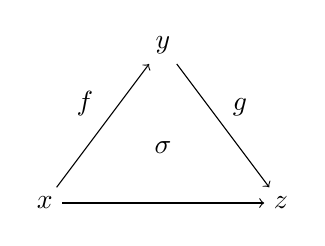
\begin{tikzpicture}[auto,->]
      \node (x) at (0,0) {$x$};
      \node (z) at (3,0) {$z$};
      \node (y) at (1.5,2) {$y$};
      \node (sigma) at (1.5,0.7) {$\sigma$};
      \draw (x) -- node {$f$} (y);
      \draw (y) -- node {$g$} (z);
      \draw (x) -- (z);  
    \end{tikzpicture}
  \]
  同様に, $X_1 \times_{X_0} X_1$は2つの合成可能な射の集まりとみなせて, 次のように表せる. 
  \[
    \begin{tikzpicture}[auto,->]
      \node (x) at (0,0) {$x$};
      \node (z) at (3,0) {$z$};
      \node (y) at (1.5,2) {$y$};
      \draw (x) -- node {$f$} (y);
      \draw (y) -- node {$g$} (z);
    \end{tikzpicture}
  \]
  Segal条件はこのような図式が次の2単体に拡張できることを意味している. 
  \[
    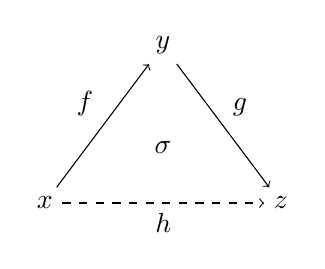
\begin{tikzpicture}[auto,->]
      \node (x) at (0,0) {$x$};
      \node (z) at (3,0) {$z$};
      \node (y) at (1.5,2) {$y$};
      \node (sigma) at (1.5,0.7) {$\sigma$};
      \draw (x) -- node {$f$} (y);
      \draw (y) -- node {$g$} (z);
      \draw[dashed] (x) -- node[swap] {$h$} (z);  
    \end{tikzpicture}
  \]
  よって, $h$を$gf$と表すことが多いが, $h$は$g$と$f$(と$\sigma$)に対して一意に定まらないことに注意. 
  しかし, \cref{theorem:composition_is_homotopic}で$h$はホモトピーの違いを除いて一意であることが分かる.  
\end{remark}

\begin{remark} \label{rem:3_segal_condition}
  $n=3$のSegal空間の条件は$\varphi_3 : X_3 \xrightarrow{\simeq} X_1 \times_{X_0} X_1 \times_{X_0} X_1$である. 
  $X_3$は3単体の集まりで, 3単体は次のように表せる. 
  \[
    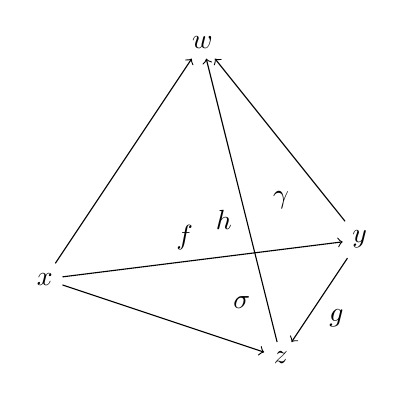
\begin{tikzpicture}[auto,->]
      \node (x) at (0,0) {$x$};
      \node (y) at (4,0.5) {$y$};
      \node (z) at (3,-1) {$z$};
      \node (w) at (2,3) {$w$};
      \node (sigma) at (2.5,-0.3) {$\sigma$};
      \node (gamma) at (3,1) {$\gamma$};
      \draw (x) -- node {$f$} (y);
      \draw (y) -- node {$g$} (z);
      \draw (z) -- node {$h$} (w);
      \draw (x) -- (z);
      \draw (x) -- (w);
      \draw (y) -- (w);
    \end{tikzpicture}
  \]
  同様に, $X_1 \times_{X_0} X_1 \times_{X_0} X_1$は3つの合成可能な射の集まりとみなせて, 次のように表せる.
  \[
    \begin{tikzpicture}[auto,->]
      \node (x) at (0,0) {$x$};
      \node (y) at (4,0.5) {$y$};
      \node (z) at (3,-1) {$z$};
      \node (w) at (2,3) {$w$};
      \draw (x) -- node {$f$} (y);
      \draw (y) -- node {$g$} (z);
      \draw (z) -- node {$h$} (w);
    \end{tikzpicture}
  \]
  Segal条件はこのような図式が次の3単体に拡張できることを意味している.
  \[
    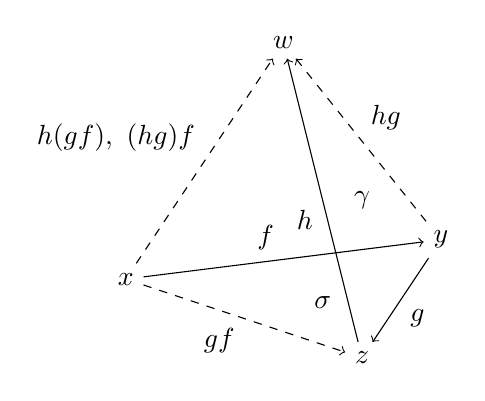
\begin{tikzpicture}[auto,->]
      \node (x) at (0,0) {$x$};
      \node (y) at (4,0.5) {$y$};
      \node (z) at (3,-1) {$z$};
      \node (w) at (2,3) {$w$};
      \node (sigma) at (2.5,-0.3) {$\sigma$};
      \node (gamma) at (3,1) {$\gamma$};
      \draw (x) -- node {$f$} (y);
      \draw (y) -- node {$g$} (z);
      \draw (z) -- node {$h$} (w);
      \draw[dashed] (x) -- node[swap] {$gf$} (z);
      \draw[dashed] (x) -- node {$h(gf),~ (hg)f$}  (w);
      \draw[dashed] (y) -- node[swap] {$hg$} (w);
    \end{tikzpicture}
  \]
  よって, この3単体は合成可能な射の結合性を表している. 
  2単体において合成は一意ではなかったが, 3単体において$(hg)f$と$h(gf)$は等しいことを意味している. 
\end{remark}

\cref{rem:2_segal_condition}と\cref{rem:3_segal_condition}で見たように, Segal条件は圏の脈体における状況と非常に似ている. 
\cref{eg:NC_is_Segal_space}で見るように, 圏の脈体はSegal空間であることが分かる. 

\begin{example} \label{eg:NC_is_Segal_space}
  任意の圏$\C$に対して, 脈体$N\C$はSegal空間である. 
\end{example}

\begin{proof}
  $N\C$が単体的集合のSegal条件を満たすことから従う.
\end{proof}

\begin{theorem}
  $X$をReedyファイブラントとする. 
  $X$がhomotopically constantのとき, $X$はSegal空間である.
\end{theorem}

% \begin{proof}
%   $X$はReedyファイブラントなので, 次の単体的集合の射
%   \begin{align*}
%     \varphi_n : X_n \to X_1 \times_{X_0} \cdots \times_{X_0} X_1
%   \end{align*}
%   は自明なKanファイブレーションである.

% \end{proof}


\section{Segal空間における射の合成} \label{sec:composition_in_Segal_space}

Segal空間とはReedyファイブラント条件とSegal条件を満たすような単体的空間であった. 
\cref{sec:segal_space}で見たように, Segal空間における射の合成は一意ではなかった (\cref{rem:2_segal_condition}).
しかし, 射の合成に関する結合律は成立していた (\cref{rem:3_segal_condition}).
この理由を考える.
$X$をSegal空間とする. 

\begin{definition}[単体的空間における対象]
  $X$をSegal空間とする. 
  $X_0$の点を$X$の対象(object)という. 
  $X$の対象の集まりを$\Ob(X)$と表すと, $\Ob(X) = T_{0,0}$である. 
\end{definition}

\begin{definition}[合成の空間]
  $X$の対象$x_0,\cdots,x_n$に対して, 単体的集合$\map_X(x_0,\cdots,x_n)$を次のpullbackで定義し, $\map_X(x_0,\cdots,x_n)$を合成の空間(space of composition)という.  
  % https://q.uiver.app/#q=WzAsNCxbMCwwLCJcXG1hcF9YKHhfMCxcXGNkb3RzLHhfbikiXSxbMSwwLCJYX24iXSxbMSwxLCIoWF8wKV57bisxfSJdLFswLDEsIlxcRGVsdGFeMCJdLFswLDFdLFswLDNdLFszLDJdLFsxLDJdLFswLDIsIiIsMSx7InN0eWxlIjp7Im5hbWUiOiJjb3JuZXIifX1dXQ==
  \[\begin{tikzcd}
    {\map_X(x_0,\cdots,x_n)} & {X_n} \\
    {\Delta^0} & {(X_0)^{n+1}=X_0 \times \cdots \times X_0}
    \arrow[from=1-1, to=1-2]
    \arrow[from=1-1, to=2-1]
    \arrow["{(x_0,\cdots,x_n)}"', from=2-1, to=2-2]
    \arrow[from=1-2, to=2-2]
    \arrow["\lrcorner"{anchor=center, pos=0.125}, draw=none, from=1-1, to=2-2]
  \end{tikzcd}\]
\end{definition}

\begin{remark}
  \cref{lem:Xn_to_X0^n+1_is_Kan_fibration}より, $X_n \to (X_0)^{n+1}$はKanファイブレーションである.
  Kanファイブレーションはpullbackで閉じるので, $\map_X(x_0,\cdots,x_n) \to \Delta^0$はKanファイブレーションである.
  つまり, $\map_X(x_0,\cdots,x_n)$はKanファイブラントである.
\end{remark}

\begin{definition}[単体的空間における射]
  合成の空間において, $n=1$のとき, 単体的集合$\map_X(x_0,x_1)$を射空間(mapping space)という. 
  $\map_X(x_0,x_1)$の点を$X$の射(morphism)といい, $f : x_0 \to x_1$と表す. 
\end{definition}

\begin{remark} \label{rem:map_is_map_times_map}
  $X$はSegal空間なので, $ X_n \to X_1 \times_{X_0} \cdots \times_{X_0} X_1$は自明なKanファイブレーションである.
  また, 合成の空間の図式は次の図式に拡張できる. 
  % https://q.uiver.app/#q=WzAsNSxbMCwwLCJcXG1hcF9YKHhfMCxcXGNkb3RzLHhfbikiXSxbMSwwLCJYX24iXSxbMSwxLCIoWF8wKV57bisxfSJdLFswLDEsIlxcRGVsdGFeMCJdLFsyLDAsIlhfMSBcXHRpbWVzX3tYXzB9IFxcdGltZXMgXFx0aW1lc197WF8wfSBYXzEiXSxbMCwxXSxbMCwzXSxbMywyLCIoeF8wLFxcY2RvdHMseF9uKSIsMl0sWzEsMl0sWzAsMiwiIiwxLHsic3R5bGUiOnsibmFtZSI6ImNvcm5lciJ9fV0sWzEsNCwiXFxjb25nIl0sWzQsMl1d
  \[\begin{tikzcd}
    {\map_X(x_0,\cdots,x_n)} & {X_n} & {X_1 \times_{X_0} \cdots \times_{X_0} X_1} \\
    {\Delta^0} & {(X_0)^{n+1}}
    \arrow[from=1-1, to=1-2]
    \arrow[from=1-1, to=2-1]
    \arrow["{(x_0,\cdots,x_n)}"', from=2-1, to=2-2]
    \arrow[from=1-2, to=2-2]
    \arrow["\lrcorner"{anchor=center, pos=0.125}, draw=none, from=1-1, to=2-2]
    \arrow["\simeq", from=1-2, to=1-3]
    \arrow[from=1-3, to=2-2]
  \end{tikzcd}\]
\end{remark}

\begin{lemma} 
  単体的集合の射
  \begin{align*}
    \map_X(x_0,\cdots,x_n) \to \map_X(x_0,x_1) \times \cdots \times \map_X(x_{n-1},x_n)
  \end{align*}
  は自明なKanファイブレーションである.
\end{lemma}

\begin{proof}
  次の図式において, 下と全体の四角はpullbackである. 
  % https://q.uiver.app/#q=WzAsNixbMCwwLCJcXGJ1bGxldFxcbWFwX1goeF8wLFxcY2RvdHMseF9uKSJdLFsxLDAsIlhfbiJdLFsxLDEsIlhfMSBcXHRpbWVzX3tYXzB9IFxcY2RvdHMgXFx0aW1lc197WF8wfSBYXzEiXSxbMSwyLCIoWF8wKV57bisxfSJdLFswLDEsIlxcbWFwX1goeF8wLHhfMSkgXFx0aW1lcyBcXGNkb3RzIFxcdGltZXMgXFxtYXBfWCh4X3tuLTF9LHhfbikiXSxbMCwyLCJcXERlbHRhXjAiXSxbMCwxXSxbMSwyLCJcXHNpbWVxIl0sWzIsM10sWzAsNF0sWzQsNV0sWzUsM10sWzQsMl1d
  \[\begin{tikzcd}
    {\bullet\map_X(x_0,\cdots,x_n)} & {X_n} \\
    {\map_X(x_0,x_1) \times \cdots \times \map_X(x_{n-1},x_n)} & {X_1 \times_{X_0} \cdots \times_{X_0} X_1} \\
    {\Delta^0} & {(X_0)^{n+1}}
    \arrow[from=1-1, to=1-2]
    \arrow["\simeq", from=1-2, to=2-2]
    \arrow[from=2-2, to=3-2]
    \arrow[from=1-1, to=2-1]
    \arrow[from=2-1, to=3-1]
    \arrow[from=3-1, to=3-2]
    \arrow[from=2-1, to=2-2]
  \end{tikzcd}\]
  よって, 上の四角もpullbackである. 
  自明なKanファイブレーションはpullbackで閉じるので, 単体的集合の射
  \begin{align*}
    \map_X(x_0,\cdots,x_n) \to \map_X(x_0,x_1) \times \cdots \times \map_X(x_{n-1},x_n)
  \end{align*}
  は自明なKanファイブレーションである.
\end{proof}

\begin{remark}
  $x,y,z$を$X$の任意の対象とする. 
  合成の空間の定義から, 次の図式が得られる. 
  % https://q.uiver.app/#q=WzAsMyxbMCwwLCJcXG1hcF9YKHgseSx6KSJdLFsxLDAsIlxcbWFwX1goeCx6KSJdLFswLDEsIlxcbWFwX1goeCx5KSBcXHRpbWVzIFxcbWFwX1goeSx6KSJdLFswLDEsImRfMSJdLFswLDIsIlxcY29uZyIsMl1d
  \[\begin{tikzcd}
    {\map_X(x,y,z)} & {\map_X(x,z)} \\
    {\map_X(x,y) \times \map_X(y,z)}
    \arrow["{d_1}", from=1-1, to=1-2]
    \arrow["\simeq"', from=1-1, to=2-1]
  \end{tikzcd}\]
  2つの射$f \in \map_X(x,y), g \in \map_X(y,z)$に対して, $\map_X(x,y,z)$の単体的部分集合$\Comp(f,g)$を次のpullbackで定義する. 
  % https://q.uiver.app/#q=WzAsNSxbMSwwLCJcXG1hcF9YKHgseSx6KSJdLFsyLDAsIlxcbWFwX1goeCx6KSJdLFsxLDEsIlxcbWFwX1goeCx5KSBcXHRpbWVzIFxcbWFwX1goeSx6KSJdLFswLDAsIlxcQ29tcChmLGcpIl0sWzAsMSwiXFxEZWx0YV4wIl0sWzAsMSwiZF8xIl0sWzAsMiwiXFxjb25nIiwyXSxbMywwLCIiLDIseyJzdHlsZSI6eyJ0YWlsIjp7Im5hbWUiOiJob29rIiwic2lkZSI6InRvcCJ9fX1dLFszLDRdLFs0LDJdLFszLDIsIiIsMSx7InN0eWxlIjp7Im5hbWUiOiJjb3JuZXIifX1dXQ==
  \[\begin{tikzcd}
    {\Comp(f,g)} & {\map_X(x,y,z)} & {\map_X(x,z)} \\
    {\Delta^0} & {\map_X(x,y) \times \map_X(y,z)}
    \arrow["{d_1}", from=1-2, to=1-3]
    \arrow["\simeq", from=1-2, to=2-2]
    \arrow[hook, from=1-1, to=1-2]
    \arrow["\simeq", from=1-1, to=2-1]
    \arrow[from=2-1, to=2-2]
    \arrow["\lrcorner"{anchor=center, pos=0.125}, draw=none, from=1-1, to=2-2]
  \end{tikzcd}\]
  自明なKanファイブレーションはpullbackで閉じるので, $\Comp(f,g) \to \Delta^0$は自明なKanファイブレーションである. 
  つまり, $\Comp(f,g)$は可縮なKanファイブラントである. 
  よって, 射の合成は可縮な空間の違いを除いて一意に定めることができる.
\end{remark}

\begin{example}
  $X$を任意の圏$\C$の脈体とする. 
  $X$の任意の対象$x,y,z$と射$f:x \to y, g: y \to z$に対して, $\Comp(f,g) \cong \Delta^0$である. 
  % このとき, 2つの射がホモトピックであることと, 2つの射が等しいことは同値である. 
  % 更に, 射がホモトピー同値であることと, 射が同型であることは同値である. 
\end{example}

\begin{proof}
  次の図式において, 同型がpullbackで閉じることから従う. 
  % https://q.uiver.app/#q=WzAsNCxbMCwwLCJcXENvbXAoZixnKSJdLFsxLDAsIk4oXFxDKV8yIl0sWzEsMSwiTihcXEMpXzEgXFx0aW1lc197TihcXEMpXzB9IE4oXFxDKV8xIl0sWzAsMSwiXFxEZWx0YV4wIl0sWzAsMV0sWzEsMiwiXFxjb25nIl0sWzAsM10sWzMsMl0sWzAsMiwiIiwxLHsic3R5bGUiOnsibmFtZSI6ImNvcm5lciJ9fV1d
  \[\begin{tikzcd}
    {\Comp(f,g)} & {N\C_2} \\
    {\Delta^0} & {N\C_1 \times_{N\C_0} N\C_1}
    \arrow[from=1-1, to=1-2]
    \arrow["\cong", from=1-2, to=2-2]
    \arrow[from=1-1, to=2-1]
    \arrow[from=2-1, to=2-2]
    \arrow["\lrcorner"{anchor=center, pos=0.125}, draw=none, from=1-1, to=2-2]
  \end{tikzcd}\]
\end{proof}

\begin{definition}[単体的空間における恒等射]
  任意の$X$の対象$x$に対して, $s_0 : X_0 \to X_1$の$x$の像$s_0(x)$を$x$の恒等射(identity map)といい, $\id_x$と表す.
  \begin{align*}
    s_0 : X_0 \to X_1 : x \mapsto \id_x
  \end{align*}
\end{definition}


\section{ホモトピー同値}

\cref{sec:composition_in_Segal_space}では主にSegal空間の圏論的な側面を見た. 
この章では, Segal空間のもつホモトピー論的な性質に着目する.
$X$をSegal空間とする. 

\begin{definition}[単体的空間におけるホモトピック]
  $x,y$を$X$の対象, $f,g \in \map_X(x,y)$を$X$の射とする.
  単体的集合の射$f,g : \Delta^0 \to \map_X(x,y)$が単体的集合の意味でホモトピックであるとき, $f$と$g$はホモトピック(homotopic)であるといい, $f \sim g$と表す.  
\end{definition}

射の合成はホモトピーの違いを除いて結合的かつ単位を持つ. 

\begin{theorem} \label{theorem:composition_is_homotopic}
  $x,y,z,w$を$X$の対象, $f \in \map_X(x,y), g \in \map_X(y,z), h \in \map_X(z,w)$を$X$の射とする. 
  このとき, $h(gf) \sim (hg)f$かつ$f\id_x \sim \id_yf \sim f$である. 
\end{theorem}

\cref{theorem:composition_is_homotopic}より, 単体的空間の対して通常の圏が定まる. 

\begin{definition}[単体的空間のホモトピー圏]
  単体的空間$X$に対して, 通常の圏$\Ho(X)$を次のように定義し, $X$のホモトピー圏(homotopy category)という. 
  \begin{itemize}
    \item $\Ho(X)$の対象は$X$の対象と同じ
    \item 任意の$x,y \in \Ho(X)$に対して, $\Hom_{\Ho(X)}(x,y)$は$x$から$y$への射のホモトピー類の空間
    \begin{align*}
      \Hom_{\Ho(X)}(x,y) := \pi_0(\map_X(x,y))
    \end{align*}
    \item 任意の$x,y,z \in \Ho(X)$に対して, 合成
    \begin{align*}
      \Hom_{\Ho(X)}(x,y) \times \Hom_{\Ho(X)}(y,z) \to \Hom_{\Ho(X)}(x,z)
    \end{align*}
    は
    \begin{align*}
      \map_X(x,y) \times \map_X(y,z) \to \map_X{\Ho(X)}(x,z)
    \end{align*}
    から定まる自然な対応
  \end{itemize}
\end{definition}

\begin{theorem} \label{thrm:C_is_HoNC}
  任意の圏$\C$は$\Ho(N\C)$と圏同型である.
\end{theorem}

\begin{proof}
  $\Ho(N\C)$の対象は
  \begin{align*}
    \Ob\Ho(N\C) = \Ob(N\C) = N\C_0 = \Ob(\C)
  \end{align*}
  任意の$x,y \in \Ho(N\C)$に対して, 
  \begin{align*}
    \Hom_{\Ho(N\C)} = \pi_0(\Map_{N\C}(x,y)) = \pi_0(N\C_1 \times_{N\C_0 \times N\C_0} \ast)
  \end{align*}
  $N\C_1$と$N\C_0 \times N\C_0$は離散的なので, 
  \begin{align*}
    \pi_0(N\C_1 \times_{N\C_0 \times N\C_0} \ast) = N\C_1 \times_{N\C_0 \times N\C_0} \ast = \Hom_\C(x,y)
  \end{align*}
  よって, $\C$と$\Ho(N\C)$は圏同型である.
\end{proof}

\begin{definition}[ホモトピー同値]
  $X$の射$f \in \map_X(x,y)$に対して, ある射$g,h \in \map_X(y,x)$が存在して, 
  \begin{align*}
    gf \sim \id_x,~ fh \sim \id_y
  \end{align*}
  を満たすとき, $f$をホモトピー同値(homotopy equivalence)という.  
  このとき, $g$を$f$の左ホモトピー逆射(left homotopy inverse), $h$を$f$の右ホモトピー逆射(right homotopy inverse)という. 
\end{definition}

ホモトピー逆射はホモトピーの違いを除いて一意である. 

\begin{remark}
  $g$を$f$の左ホモトピー逆射, $h$を$f$の右ホモトピー逆射とする. 
  \cref{theorem:composition_is_homotopic}より, 
  \begin{align*}
    g \sim g \id_y \sim g f h \sim \id_x h \sim h
  \end{align*}
  なので, ホモトピー逆射はホモトピーの違いを除いて一意である. 
\end{remark}

\begin{example} \label{eg:id_is_homotopy_equivalence}
  $X$の任意の対象$x$に対して, $x$の恒等射$\id_x$はホモトピー逆射である.
\end{example}

ホモトピー同値がホモトピーに関して保たれることを見るために, いくつか準備をする.

\begin{definition}
  $Z(3)$を次の図式の余極限で定まる$F(3)$の単体的部分空間とする. 
  % https://q.uiver.app/#q=WzAsNSxbMCwwLCJGKDEpIl0sWzEsMSwiRigwKSJdLFsyLDAsIkYoMSkiXSxbMywxLCJGKDApIl0sWzQsMCwiRigxKSJdLFsxLDAsIjEiXSxbMSwyLCIxIiwyXSxbMywyLCIwIl0sWzMsNCwiMCIsMl1d
  \[\begin{tikzcd}
    {F(1)} && {F(1)} && {F(1)} \\
    & {F(0)} && {F(0)}
    \arrow["1", from=2-2, to=1-1]
    \arrow["1"', from=2-2, to=1-3]
    \arrow["0", from=2-4, to=1-3]
    \arrow["0"', from=2-4, to=1-5]
  \end{tikzcd}\]
\end{definition}

\begin{remark}
  単体的空間$Z(3)$に対して, $\Map_\sSpace(Z(3),X)$は次の極限
  \begin{align*}
    \Map_\sSpace(Z(3),X) \cong X_1 \times_{X_0} X_1 \times_{X_0} X_1
  \end{align*}
  で表され, 次の図式の極限として表せる. 
  % https://q.uiver.app/#q=WzAsNSxbMCwwLCJYXzEiXSxbMSwxLCJYXzAiXSxbMiwwLCJYXzEiXSxbMywxLCJYXzAiXSxbNCwwLCJYXzEiXSxbMCwxLCJkXzEiLDJdLFsyLDEsImRfMSJdLFsyLDMsImRfMCIsMl0sWzQsMywiZF8wIl1d
  \[\begin{tikzcd}
    {X_1} && {X_1} && {X_1} \\
    & {X_0} && {X_0}
    \arrow["{d_1}"', from=1-1, to=2-2]
    \arrow["{d_1}", from=1-3, to=2-2]
    \arrow["{d_0}"', from=1-3, to=2-4]
    \arrow["{d_0}", from=1-5, to=2-4]
  \end{tikzcd}\]

\end{remark}

\begin{lemma}
  $f,g \in X_1$を$X$の射とする. 
  ある$\gamma : \Delta^1 \to X_1$が存在して, $\gamma(0)=f, \gamma(1)=g$を満たすとする. 
  $g$がホモトピー同値のとき, $f$もホモトピー同値である. 
\end{lemma}

\begin{definition}[ホモトピー同値の空間]
  $X$のホモトピー同値で生成される$X_1$の単体的部分空間を$X_\hoequiv$と表し, $X$のホモトピー同値の空間(space of homotopy equivalences)という. 
\end{definition}

\begin{remark}
  $X_\hoequiv$の点は$X$の射である.
  具体的には, $X_\hoequiv$はホモトピー逆射が存在するような$X$の射のなす$X_1$の充満部分空間である.  
\end{remark}

ホモトピー同値の空間は可縮である. 
つまり, 射がホモトピー同値となるような逆射の選択はホモトピーの違いを除いて一意である. 

\begin{lemma}
  $X$のホモトピー同値$f$, $f$の左ホモトピー逆射$g$, $f$の右ホモトピー逆射$h$の3つ組$(f,g,h)$で生成される$X_3$の単体的部分空間を$X_\hoeqchoice$と表す. 
  $U : X_\hoeqchoice \to X_\hoequiv : (f,g,h) \mapsto f$をホモトピー逆射を忘れる射とする. 
  このとき, $U$は次の図式を可換にする自明なKanファイブレーションである. 
  % https://q.uiver.app/#q=WzAsMyxbMCwwLCJYX1xcaG9lcXVpdiJdLFsxLDAsIlhfXFxob2VxY2hvaWNlIl0sWzEsMSwiWF8xIl0sWzEsMCwiVSIsMl0sWzEsMl0sWzAsMiwiIiwyLHsic3R5bGUiOnsidGFpbCI6eyJuYW1lIjoiaG9vayIsInNpZGUiOiJ0b3AifX19XV0=
  \[\begin{tikzcd}
    {X_\hoequiv} & {X_\hoeqchoice} \\
    & {X_1}
    \arrow["U"', from=1-2, to=1-1]
    \arrow[from=1-2, to=2-2]
    \arrow[hook, from=1-1, to=2-2]
  \end{tikzcd}\]
  また, 次のpullbackが存在する.
  % https://q.uiver.app/#q=WzAsNSxbMCwwLCJYX1xcaG9lcXVpdiJdLFsxLDAsIlhfXFxob2VxY2hvaWNlIl0sWzEsMSwiWF8xIl0sWzIsMCwiWF8zIl0sWzIsMSwiWF8xIFxcdGltZXNfe1hfMH1YXzEgXFx0aW1lc197WF8wfSBYXzEiXSxbMSwwLCJcXGNvbmciLDJdLFsxLDJdLFswLDIsIiIsMix7InN0eWxlIjp7InRhaWwiOnsibmFtZSI6Imhvb2siLCJzaWRlIjoidG9wIn19fV0sWzEsMywiIiwyLHsic3R5bGUiOnsidGFpbCI6eyJuYW1lIjoiaG9vayIsInNpZGUiOiJ0b3AifX19XSxbMyw0LCIoZF8xZF8zLGRfMGRfMyxkXzFkXzApIl0sWzIsNCwiKHNfMGRfMCxcXGlkX3t4XzF9LHNfMGRfMSkiLDJdLFsxLDQsIiIsMCx7InN0eWxlIjp7Im5hbWUiOiJjb3JuZXIifX1dXQ==
  \[\begin{tikzcd}
    {X_\hoequiv} & {X_\hoeqchoice} & {X_3} \\
    & {X_1} & {X_1 \times_{X_0}X_1 \times_{X_0} X_1}
    \arrow["\cong"', from=1-2, to=1-1]
    \arrow[from=1-2, to=2-2]
    \arrow[hook, from=1-1, to=2-2]
    \arrow[hook, from=1-2, to=1-3]
    \arrow["{(d_1d_3,d_0d_3,d_1d_0)}", from=1-3, to=2-3]
    \arrow["{(s_0d_0,\id_{x_1},s_0d_1)}"', from=2-2, to=2-3]
    \arrow["\lrcorner"{anchor=center, pos=0.125}, draw=none, from=1-2, to=2-3]
  \end{tikzcd}\] 
\end{lemma}

ホモトピー同値を用いて定義される空間として, 次の2つが重要である. 

\begin{definition}[Segal空間亜群]
  $X$の任意の射がホモトピー同値のとき, $X$をSegal空間亜群(Segal space groupoid)という. 
\end{definition}

局所的なホモトピー同値の定義を与える. 

\begin{definition}[$x$と$y$の間のホモトピー同値の空間]
  $x,y$を$X$の対象とする. 
  単体的集合$\hoequiv_X(x,y)$を次のpullbackで定義し, $x$と$y$の間のホモトピー同値の空間(space of homotopy equivalences between two objects $x$ and $y$)という. 
  % https://q.uiver.app/#q=WzAsNCxbMCwwLCJcXGhvZXF1aXZfWCh4LHkpIl0sWzEsMCwiWF9cXGhvZXF1aXYiXSxbMSwxLCJYXzAgXFx0aW1lcyBYXzAiXSxbMCwxLCJcXERlbHRhXjAiXSxbMCwxXSxbMSwyLCIoZF8wLGRfMSkiXSxbMCwzXSxbMywyLCIoeCx5KSIsMl0sWzAsMiwiIiwxLHsic3R5bGUiOnsibmFtZSI6ImNvcm5lciJ9fV1d
  \[\begin{tikzcd}
    {\hoequiv_X(x,y)} & {X_\hoequiv} \\
    {\Delta^0} & {X_0 \times X_0}
    \arrow[from=1-1, to=1-2]
    \arrow["{(d_0,d_1)}", from=1-2, to=2-2]
    \arrow[from=1-1, to=2-1]
    \arrow["{(x,y)}"', from=2-1, to=2-2]
    \arrow["\lrcorner"{anchor=center, pos=0.125}, draw=none, from=1-1, to=2-2]
  \end{tikzcd}\]
\end{definition}

\begin{example} \label{eg:homotopy_equivalence_is_isomorphism_in_NC}
  $\C$を通常の圏とする. 
  脈体$N\C$におけるホモトピー同値は$\C$における同型射である. 
\end{example}

\begin{proof}
  $N\C$において射$f$がホモトピー同値であることと, $\Ho(N\C)$において射$[f]$が同型射であることは同値である. 
  \cref{thrm:C_is_HoNC}より, $\Ho(N\C) = \C$である. 
  よって, $N\C$において射$f$がホモトピー同値であることと, $\C$において射$[f]$が同型射であることは同値である. 
\end{proof}

\section{完備Segal空間} \label{sec:complete_segal_space}

\cref{sec:reedy_fibrant}と\cref{sec:segal_space}でSegal空間がホモトピー論と圏論の2つの性質を持つことを見た. 
しかし, Segal空間のホモトピー論と圏論は次で見るように整合性がない.

\begin{definition}
  $I(1)$を2つの対象$x,y$とその間の可逆な射からなる圏とする. 
  \footnote{
    恒等射はもちろん存在するが, 恒等射は明記しない. 
  }
  % https://q.uiver.app/#q=WzAsMixbMCwwLCJ4Il0sWzEsMCwieSJdLFswLDEsImYiLDAseyJvZmZzZXQiOi0xfV0sWzEsMCwiZl57LTF9IiwwLHsib2Zmc2V0IjotMX1dXQ==
  \[\begin{tikzcd}
    x & y
    \arrow["f", shift left, from=1-1, to=1-2]
    \arrow["{f^{-1}}", shift left, from=1-2, to=1-1]
  \end{tikzcd}\]
\end{definition}

\begin{remark} \label{rem:E(1)}
  Segal空間$i_F^\ast(NI(1))$を$E(1)$と表す. 
  $E(1)$は離散単体的空間なので, 任意の$n$に対して, 
  \begin{align*}
    E(1)_n = \{x,y\}^n
  \end{align*}
  である. 
  具体的には, $E(1)_n$は集合$\{0,\cdots,n-1\}$から$\{x,y\}$への射の集まりである. 
  よって, $E(1)_n$は$2^{n+1}$個の元を持つ.
  例えば, $E(1)_0$は$\{x,y\}$である. 
  また, $E(1)_1$は$\{\id_x,\id_y, f, f^{-1}\}$である. 
\end{remark}

\begin{lemma}
  圏$I(1)$と$\{\ast\}$は圏同値である. 
  しかし, $E(1) := i_F^\ast(NI(1))$と$F(1) := i_F^\ast(N\{\ast\})$はSegal空間として圏同値ではない.
\end{lemma}

\begin{proof}
  $E(1)$は各次元で可縮ではないが, $F(1)$は各次元で可縮であることから, 明らかにSegal空間として圏同値でない.
\end{proof}

Segal空間のホモトピー論と圏論に整合性を持たせる条件が完備性である. 

\begin{remark}
  単体的空間$X$に対して, ホモトピー同値の空間$X_\hoequiv \subset X_1$が存在する. 
  恒等射の定義
  \begin{align*}
    s_0 : X_0 \to X_1 : x \mapsto \id_x
  \end{align*}
  において, \cref{eg:id_is_homotopy_equivalence}より, 恒等射はホモトピー同値である. 
  よって, $s_0$は$X_\hoequiv$を経由して分解される. 
  % https://q.uiver.app/#q=WzAsMyxbMCwwLCJYXzAiXSxbMiwwLCJYXzEiXSxbMSwxLCJYX1xcaG9lcXVpdiJdLFswLDEsInNfMCJdLFswLDJdLFsyLDEsIiIsMix7InN0eWxlIjp7InRhaWwiOnsibmFtZSI6Imhvb2siLCJzaWRlIjoidG9wIn19fV1d
\[\begin{tikzcd}
	{X_0} && {X_1} \\
	& {X_\hoequiv}
	\arrow["{s_0}", from=1-1, to=1-3]
	\arrow[from=1-1, to=2-2]
	\arrow[hook, from=2-2, to=1-3]
\end{tikzcd}\]
\end{remark}

単体的空間の射$s_0 : X_0 \to X_1$は単射ではあるが, 全射ではない. 
($X_1$の任意の同型射が恒等射のみであるとき, $s_0$は全射である.)
よって, 完備Segal空間は次のように定義される. 

\begin{definition}[完備Segal空間]
  $X$をSegal空間とする.
  単体的集合の射
  \begin{align*}
    s_0 : X_0 \to X_\hoequiv
  \end{align*}
  が弱同値のとき, $X$を完備Segal空間(complete Segal space)という. 
\end{definition}

\begin{example}
  単体的空間$E(1)$は完備Segal空間ではない.
\end{example}

\begin{proof}
  \cref{rem:E(1)}より, 
  \begin{align*}
    E(1)_0 &= \{x,y\} \\
    E(1)_1 &= \{\id_x,\id_y, f, f^{-1}\} \\
    E(1)_\hoequiv &= \{\id_x,\id_y, f, f^{-1}\} = E(1)_1
  \end{align*}
  であるが, 
  \begin{align*}
    E(1)_0 \to E(1)_\hoequiv = \{x,y\} \to \{\id_x,\id_y, f, f^{-1}\}
  \end{align*}
  は弱同値ではない. 
  よって, $E(1)$は完備Segal空間ではない.
\end{proof}

完備Segal空間の定義と同値な条件がある. 

\begin{theorem}
  単体的空間$X$に対して, 次は同値である. 
  \begin{enumerate}
    \item $X$は完備Segal空間である. 
    \item 次の図式はホモトピーpullbackである. 
    % https://q.uiver.app/#q=WzAsNCxbMCwwLCJYXzAiXSxbMSwwLCJYXzMiXSxbMCwxLCJYXzEiXSxbMSwxLCJYXzEgXFx0aW1lc197WF8wfSBYXzEgXFx0aW1lc197WF8wfSBYXzEiXSxbMCwxXSxbMCwyXSxbMSwzXSxbMiwzXSxbMCwzLCIiLDEseyJzdHlsZSI6eyJuYW1lIjoiY29ybmVyIn19XV0=
    \[\begin{tikzcd}
      {X_0} & {X_3} \\
      {X_1} & {X_1 \times_{X_0} X_1 \times_{X_0} X_1}
      \arrow[from=1-1, to=1-2]
      \arrow[from=1-1, to=2-1]
      \arrow[from=1-2, to=2-2]
      \arrow[from=2-1, to=2-2]
      \arrow["\lrcorner"{anchor=center, pos=0.125}, draw=none, from=1-1, to=2-2]
    \end{tikzcd}\]
    \item 次の単体的空間の射は弱同値である. 
    \begin{align*}
      \Map_\sSpace(E(1),X) \to \Map_\sSpace(F(0),X)
    \end{align*}
    \item 任意の対象$x,y \in X$に対して, $x$と$y$の間のホモトピー同値の空間$\hoequiv_X(x,y)$は$x$から$y$への$X_0$における道の空間と弱同値である. 
  \end{enumerate}
\end{theorem}

完備Segal空間の条件をまとめる. 

\begin{remark}
  完備Segal空間は次の条件を満たす単体的空間である. 
  \begin{description}
    \item[(Reedyファイブラント条件)] 垂直な軸はホモトピー論の性質をもつ. 
    \item[(Segal条件)] 水平な軸は圏論的な性質をもつ. 
    \item[(完備性)] ホモトピー論の性質と圏論の性質は整合的である.  
  \end{description}
\end{remark}

Segal空間亜群の完備性も定義できる. 

\begin{definition}[完備Segal空間亜群]
  $X$を完備Segal空間とする. 
  $X$の任意の射がホモトピー同値のとき, $X$を完備Segal空間亜群(complete Segal space groupoid)という.
\end{definition}

\begin{theorem} \label{thrm:NC_is_complete_equals_has_non_trivial_morphism}
  $\C$を通常の圏とする. 
  脈体$N\C$が完備Segal空間であることと, $\C$が恒等射以外の同型射を持たないことは同値である. 
\end{theorem}

\begin{proof}
  ($\Rightarrow$) : $N\C$が完備Segal空間であるとする. 
  このとき, 単体的空間の射
  \begin{align*}
    N\C_0 \to N^C_\hoequiv
  \end{align*}
  は弱同値である. 
  $N\C_0$と$NC_\hoequiv$は離散的なので, 
  \begin{align*}
    N\C_0 \to NC_\hoequiv
  \end{align*}
  は集合の全単射である. 
  よって, 恒等射以外のホモトピー同値は存在しない. 
  \cref{eg:homotopy_equivalence_is_isomorphism_in_NC}より, $N\C$におけるホモトピー同値は$\C$における同型射である.
  よって, $\C$は恒等射以外の同型射を持たない.

  ($\Leftarrow$) : $\C$が恒等射以外の同型射を持たないとすると, 
  \begin{align*}
    N\C_0 \to N\C_\hoequiv = \Iso\C : x \mapsto \id_x
  \end{align*}
  は集合の全単射である. 
  よって, ホモトピー同値である. 
  従って, 脈体$N\C$は完備Segal空間である.
\end{proof}

\cref{thrm:NC_is_complete_equals_has_non_trivial_morphism}より, 通常の圏$\C$が恒等射以外の同型射を持つとき, 単体的集合の脈体ではうまくいかない.
そのため, 圏のホモトピー論を考慮するような脈体として, 圏の分類図式と呼ばれる概念を定義する. 

% \begin{definition}[核]
  
% \end{definition}

\begin{definition}[分類図式]
  $\C$を通常の圏とする. 
  単体的空間$\N\C$を任意の$n,l \geq 0$に対して次のように定義し, $\C$の分類図式(classifying diagram)という. 
  \begin{align*}
    \N\C_{n,l} &:= \Hom_\Cat([n] \times I(l), \C) \\
    \N\C_n &:= N(\Fun([n],\C)^\core)
  \end{align*}
\end{definition}

\begin{remark}
  $\C$の分類図式において, $n=0$のとき, 
  \begin{align*}
    \N\C_0 = N(\Fun([0],\C)^\core) = N(\C^\core)
  \end{align*}
\end{remark}

\begin{remark}
  $\C$の分類図式は次のように表せる. 
  % https://q.uiver.app/#q=WzAsMjQsWzAsMCwiXFxOXFxDX3swLDB9Il0sWzEsMCwiXFxOXFxDX3sxLDB9Il0sWzAsMSwiXFxOXFxDX3swLDF9Il0sWzEsMSwiXFxOXFxDX3sxLDF9Il0sWzAsMiwiXFxOXFxDX3swLDJ9Il0sWzEsMiwiXFxOXFxDX3sxLDJ9Il0sWzIsMCwiXFxOXFxDX3syLDB9Il0sWzIsMSwiXFxOXFxDX3syLDF9Il0sWzIsMiwiXFxOXFxDX3syLDJ9Il0sWzMsMCwiXFxjZG90cyJdLFs0LDAsIlxcTlxcQ197LSwwfSJdLFszLDEsIlxcY2RvdHMiXSxbNCwxLCJcXE5cXENfey0sMX0iXSxbMywyLCJcXGNkb3RzIl0sWzQsMiwiXFxOXFxDX3stLDJ9Il0sWzAsMywiXFx2ZG90cyJdLFsxLDMsIlxcdmRvdHMiXSxbMiwzLCJcXHZkb3RzIl0sWzAsNCwiXFxDXlxcY29yZSJdLFsxLDQsIlxcRnVuKFsxXSxcXEMpXlxcY29yZSJdLFsyLDQsIlxcRnVuKFsyXSxcXEMpXlxcY29yZSJdLFs0LDMsIlxcdmRvdHMiXSxbMyw0LCJcXGNkb3RzIl0sWzMsMywiXFxkZG90cyJdLFswLDFdLFsxLDAsIiIsMix7Im9mZnNldCI6MX1dLFsxLDAsIiIsMSx7Im9mZnNldCI6LTF9XSxbMCwyXSxbMiwzXSxbMSwzXSxbMiwwLCIiLDEseyJvZmZzZXQiOjF9XSxbMiwwLCIiLDEseyJvZmZzZXQiOi0xfV0sWzMsMSwiIiwxLHsib2Zmc2V0IjoxfV0sWzMsMSwiIiwxLHsib2Zmc2V0IjotMX1dLFszLDIsIiIsMSx7Im9mZnNldCI6MX1dLFszLDIsIiIsMSx7Im9mZnNldCI6LTF9XSxbNCwyXSxbNCwyLCIiLDEseyJvZmZzZXQiOi0yfV0sWzUsM10sWzIsNCwiIiwxLHsib2Zmc2V0IjoxfV0sWzIsNCwiIiwxLHsib2Zmc2V0IjotMX1dLFs0LDIsIiIsMSx7Im9mZnNldCI6Mn1dLFs0LDVdLFs1LDQsIiIsMSx7Im9mZnNldCI6LTF9XSxbMyw1LCIiLDEseyJvZmZzZXQiOjF9XSxbMyw1LCIiLDEseyJvZmZzZXQiOi0xfV0sWzUsMywiIiwxLHsib2Zmc2V0IjoyfV0sWzUsMywiIiwxLHsib2Zmc2V0IjotMn1dLFs2LDFdLFsxLDYsIiIsMSx7Im9mZnNldCI6LTF9XSxbMSw2LCIiLDEseyJvZmZzZXQiOjF9XSxbNiwxLCIiLDEseyJvZmZzZXQiOjJ9XSxbNiwxLCIiLDEseyJvZmZzZXQiOi0yfV0sWzcsM10sWzMsNywiIiwxLHsib2Zmc2V0IjoxfV0sWzMsNywiIiwxLHsib2Zmc2V0IjotMX1dLFs3LDMsIiIsMSx7Im9mZnNldCI6Mn1dLFs3LDMsIiIsMSx7Im9mZnNldCI6LTJ9XSxbNiw3XSxbNyw2LCIiLDEseyJvZmZzZXQiOjF9XSxbNyw2LCIiLDEseyJvZmZzZXQiOi0xfV0sWzgsN10sWzcsOCwiIiwxLHsib2Zmc2V0IjoxfV0sWzcsOCwiIiwxLHsib2Zmc2V0IjotMX1dLFs4LDcsIiIsMSx7Im9mZnNldCI6Mn1dLFs4LDcsIiIsMSx7Im9mZnNldCI6LTJ9XSxbOCw1XSxbNSw4LCIiLDEseyJvZmZzZXQiOjF9XSxbNSw4LCIiLDEseyJvZmZzZXQiOi0xfV0sWzgsNSwiIiwxLHsib2Zmc2V0IjoyfV0sWzgsNSwiIiwxLHsib2Zmc2V0IjotMn1dLFsxOCwxOV0sWzE5LDE4LCIiLDEseyJvZmZzZXQiOjF9XSxbMjAsMTldLFsxOSwyMCwiIiwxLHsib2Zmc2V0IjoxfV0sWzE5LDE4LCIiLDEseyJvZmZzZXQiOi0xfV0sWzE5LDIwLCIiLDEseyJvZmZzZXQiOi0xfV0sWzIwLDE5LCIiLDEseyJvZmZzZXQiOjJ9XSxbMjAsMTksIiIsMSx7Im9mZnNldCI6LTJ9XSxbMTAsMTJdLFsxMiwxMCwiIiwxLHsib2Zmc2V0IjoxfV0sWzEyLDEwLCIiLDEseyJvZmZzZXQiOi0xfV0sWzE0LDEyXSxbMTIsMTQsIiIsMSx7Im9mZnNldCI6MX1dLFsxMiwxNCwiIiwxLHsib2Zmc2V0IjotMX1dLFsxNCwxMiwiIiwxLHsib2Zmc2V0IjoyfV0sWzE0LDEyLCIiLDEseyJvZmZzZXQiOi0yfV0sWzYsOV0sWzksNiwiIiwxLHsib2Zmc2V0IjoxfV0sWzksNiwiIiwxLHsib2Zmc2V0IjotMX1dLFs2LDksIiIsMSx7Im9mZnNldCI6Mn1dLFs2LDksIiIsMSx7Im9mZnNldCI6LTJ9XSxbOSw2LCIiLDEseyJvZmZzZXQiOjN9XSxbOSw2LCIiLDEseyJvZmZzZXQiOi0zfV0sWzcsMTFdLFsxMSw3LCIiLDEseyJvZmZzZXQiOi0xfV0sWzExLDcsIiIsMSx7Im9mZnNldCI6MX1dLFs3LDExLCIiLDEseyJvZmZzZXQiOjJ9XSxbNywxMSwiIiwxLHsib2Zmc2V0IjotMn1dLFsxMSw3LCIiLDEseyJvZmZzZXQiOjN9XSxbMTEsNywiIiwxLHsib2Zmc2V0IjotM31dLFs4LDEzXSxbMTMsOCwiIiwxLHsib2Zmc2V0IjoxfV0sWzEzLDgsIiIsMSx7Im9mZnNldCI6LTF9XSxbOCwxMywiIiwxLHsib2Zmc2V0IjoyfV0sWzgsMTMsIiIsMSx7Im9mZnNldCI6LTJ9XSxbMTMsOCwiIiwxLHsib2Zmc2V0IjozfV0sWzEzLDgsIiIsMSx7Im9mZnNldCI6LTN9XSxbOSwxMCwiIiwxLHsic3R5bGUiOnsiaGVhZCI6eyJuYW1lIjoibm9uZSJ9fX1dLFsxMCw5LCIiLDEseyJvZmZzZXQiOjEsInN0eWxlIjp7ImhlYWQiOnsibmFtZSI6Im5vbmUifX19XSxbMTEsMTIsIiIsMSx7InN0eWxlIjp7ImhlYWQiOnsibmFtZSI6Im5vbmUifX19XSxbMTIsMTEsIiIsMSx7Im9mZnNldCI6MSwic3R5bGUiOnsiaGVhZCI6eyJuYW1lIjoibm9uZSJ9fX1dLFsxMywxNCwiIiwxLHsic3R5bGUiOnsiaGVhZCI6eyJuYW1lIjoibm9uZSJ9fX1dLFsxNCwxMywiIiwxLHsib2Zmc2V0IjoxLCJzdHlsZSI6eyJoZWFkIjp7Im5hbWUiOiJub25lIn19fV0sWzQsMTVdLFsxNSw0LCIiLDEseyJvZmZzZXQiOjF9XSxbMTUsNCwiIiwxLHsib2Zmc2V0IjotMX1dLFs0LDE1LCIiLDEseyJvZmZzZXQiOjJ9XSxbNCwxNSwiIiwxLHsib2Zmc2V0IjotMn1dLFsxNSw0LCIiLDEseyJvZmZzZXQiOi0zfV0sWzUsMTZdLFsxNiw1LCIiLDEseyJvZmZzZXQiOjF9XSxbMTYsNSwiIiwxLHsib2Zmc2V0IjotMX1dLFs1LDE2LCIiLDEseyJvZmZzZXQiOjJ9XSxbNSw0LCIiLDEseyJvZmZzZXQiOjF9XSxbNSwxNiwiIiwxLHsib2Zmc2V0IjotMn1dLFsxNiw1LCIiLDEseyJvZmZzZXQiOjN9XSxbMTYsNSwiIiwxLHsib2Zmc2V0IjotM31dLFsxNSw0LCIiLDEseyJvZmZzZXQiOjN9XSxbMTUsMTgsIiIsMSx7InN0eWxlIjp7ImhlYWQiOnsibmFtZSI6Im5vbmUifX19XSxbMTUsMTgsIiIsMSx7Im9mZnNldCI6MSwic3R5bGUiOnsiaGVhZCI6eyJuYW1lIjoibm9uZSJ9fX1dLFsxNiwxOSwiIiwxLHsic3R5bGUiOnsiaGVhZCI6eyJuYW1lIjoibm9uZSJ9fX1dLFsxNiwxOSwiIiwxLHsib2Zmc2V0IjoxLCJzdHlsZSI6eyJoZWFkIjp7Im5hbWUiOiJub25lIn19fV0sWzE3LDIwLCIiLDEseyJzdHlsZSI6eyJoZWFkIjp7Im5hbWUiOiJub25lIn19fV0sWzE3LDIwLCIiLDEseyJvZmZzZXQiOjEsInN0eWxlIjp7ImhlYWQiOnsibmFtZSI6Im5vbmUifX19XSxbOCwxN10sWzE3LDgsIiIsMSx7Im9mZnNldCI6MX1dLFsxNyw4LCIiLDEseyJvZmZzZXQiOi0xfV0sWzgsMTcsIiIsMSx7Im9mZnNldCI6Mn1dLFs4LDE3LCIiLDEseyJvZmZzZXQiOi0yfV0sWzE3LDgsIiIsMSx7Im9mZnNldCI6M31dLFsxNyw4LCIiLDEseyJvZmZzZXQiOi0zfV0sWzIwLDIyXSxbMjMsMjIsIiIsMSx7InN0eWxlIjp7ImhlYWQiOnsibmFtZSI6Im5vbmUifX19XSxbMjMsMjIsIiIsMSx7Im9mZnNldCI6MSwic3R5bGUiOnsiaGVhZCI6eyJuYW1lIjoibm9uZSJ9fX1dLFsyMywyMSwiIiwxLHsic3R5bGUiOnsiaGVhZCI6eyJuYW1lIjoibm9uZSJ9fX1dLFsyMywyMSwiIiwxLHsib2Zmc2V0IjotMSwic3R5bGUiOnsiaGVhZCI6eyJuYW1lIjoibm9uZSJ9fX1dLFsxNCwyMV0sWzIxLDE0LCIiLDEseyJvZmZzZXQiOjF9XSxbMjEsMTQsIiIsMSx7Im9mZnNldCI6LTF9XSxbMTQsMjEsIiIsMSx7Im9mZnNldCI6Mn1dLFsxNCwyMSwiIiwxLHsib2Zmc2V0IjotMn1dLFsyMSwxNCwiIiwxLHsib2Zmc2V0IjozfV0sWzIxLDE0LCIiLDEseyJvZmZzZXQiOi0zfV0sWzIyLDIwLCIiLDEseyJvZmZzZXQiOjF9XSxbMjIsMjAsIiIsMSx7Im9mZnNldCI6LTF9XSxbMjAsMjIsIiIsMSx7Im9mZnNldCI6Mn1dLFsyMCwyMiwiIiwxLHsib2Zmc2V0IjotMn1dLFsyMiwyMCwiIiwxLHsib2Zmc2V0IjozfV0sWzIyLDIwLCIiLDEseyJvZmZzZXQiOi0zfV1d
  \[\begin{tikzcd}
    {\N\C_{0,0}} & {\N\C_{1,0}} & {\N\C_{2,0}} & \cdots & {\N\C_{-,0}} \\
    {\N\C_{0,1}} & {\N\C_{1,1}} & {\N\C_{2,1}} & \cdots & {\N\C_{-,1}} \\
    {\N\C_{0,2}} & {\N\C_{1,2}} & {\N\C_{2,2}} & \cdots & {\N\C_{-,2}} \\
    \vdots & \vdots & \vdots & \ddots & \vdots \\
    {\C^\core} & {\Fun([1],\C)^\core} & {\Fun([2],\C)^\core} & \cdots
    \arrow[from=1-1, to=1-2]
    \arrow[shift right, from=1-2, to=1-1]
    \arrow[shift left, from=1-2, to=1-1]
    \arrow[from=1-1, to=2-1]
    \arrow[from=2-1, to=2-2]
    \arrow[from=1-2, to=2-2]
    \arrow[shift right, from=2-1, to=1-1]
    \arrow[shift left, from=2-1, to=1-1]
    \arrow[shift right, from=2-2, to=1-2]
    \arrow[shift left, from=2-2, to=1-2]
    \arrow[shift right, from=2-2, to=2-1]
    \arrow[shift left, from=2-2, to=2-1]
    \arrow[from=3-1, to=2-1]
    \arrow[shift left=2, from=3-1, to=2-1]
    \arrow[from=3-2, to=2-2]
    \arrow[shift right, from=2-1, to=3-1]
    \arrow[shift left, from=2-1, to=3-1]
    \arrow[shift right=2, from=3-1, to=2-1]
    \arrow[from=3-1, to=3-2]
    \arrow[shift left, from=3-2, to=3-1]
    \arrow[shift right, from=2-2, to=3-2]
    \arrow[shift left, from=2-2, to=3-2]
    \arrow[shift right=2, from=3-2, to=2-2]
    \arrow[shift left=2, from=3-2, to=2-2]
    \arrow[from=1-3, to=1-2]
    \arrow[shift left, from=1-2, to=1-3]
    \arrow[shift right, from=1-2, to=1-3]
    \arrow[shift right=2, from=1-3, to=1-2]
    \arrow[shift left=2, from=1-3, to=1-2]
    \arrow[from=2-3, to=2-2]
    \arrow[shift right, from=2-2, to=2-3]
    \arrow[shift left, from=2-2, to=2-3]
    \arrow[shift right=2, from=2-3, to=2-2]
    \arrow[shift left=2, from=2-3, to=2-2]
    \arrow[from=1-3, to=2-3]
    \arrow[shift right, from=2-3, to=1-3]
    \arrow[shift left, from=2-3, to=1-3]
    \arrow[from=3-3, to=2-3]
    \arrow[shift right, from=2-3, to=3-3]
    \arrow[shift left, from=2-3, to=3-3]
    \arrow[shift right=2, from=3-3, to=2-3]
    \arrow[shift left=2, from=3-3, to=2-3]
    \arrow[from=3-3, to=3-2]
    \arrow[shift right, from=3-2, to=3-3]
    \arrow[shift left, from=3-2, to=3-3]
    \arrow[shift right=2, from=3-3, to=3-2]
    \arrow[shift left=2, from=3-3, to=3-2]
    \arrow[from=5-1, to=5-2]
    \arrow[shift right, from=5-2, to=5-1]
    \arrow[from=5-3, to=5-2]
    \arrow[shift right, from=5-2, to=5-3]
    \arrow[shift left, from=5-2, to=5-1]
    \arrow[shift left, from=5-2, to=5-3]
    \arrow[shift right=2, from=5-3, to=5-2]
    \arrow[shift left=2, from=5-3, to=5-2]
    \arrow[from=1-5, to=2-5]
    \arrow[shift right, from=2-5, to=1-5]
    \arrow[shift left, from=2-5, to=1-5]
    \arrow[from=3-5, to=2-5]
    \arrow[shift right, from=2-5, to=3-5]
    \arrow[shift left, from=2-5, to=3-5]
    \arrow[shift right=2, from=3-5, to=2-5]
    \arrow[shift left=2, from=3-5, to=2-5]
    \arrow[from=1-3, to=1-4]
    \arrow[shift right, from=1-4, to=1-3]
    \arrow[shift left, from=1-4, to=1-3]
    \arrow[shift right=2, from=1-3, to=1-4]
    \arrow[shift left=2, from=1-3, to=1-4]
    \arrow[shift right=3, from=1-4, to=1-3]
    \arrow[shift left=3, from=1-4, to=1-3]
    \arrow[from=2-3, to=2-4]
    \arrow[shift left, from=2-4, to=2-3]
    \arrow[shift right, from=2-4, to=2-3]
    \arrow[shift right=2, from=2-3, to=2-4]
    \arrow[shift left=2, from=2-3, to=2-4]
    \arrow[shift right=3, from=2-4, to=2-3]
    \arrow[shift left=3, from=2-4, to=2-3]
    \arrow[from=3-3, to=3-4]
    \arrow[shift right, from=3-4, to=3-3]
    \arrow[shift left, from=3-4, to=3-3]
    \arrow[shift right=2, from=3-3, to=3-4]
    \arrow[shift left=2, from=3-3, to=3-4]
    \arrow[shift right=3, from=3-4, to=3-3]
    \arrow[shift left=3, from=3-4, to=3-3]
    \arrow[no head, from=1-4, to=1-5]
    \arrow[shift right, no head, from=1-5, to=1-4]
    \arrow[no head, from=2-4, to=2-5]
    \arrow[shift right, no head, from=2-5, to=2-4]
    \arrow[no head, from=3-4, to=3-5]
    \arrow[shift right, no head, from=3-5, to=3-4]
    \arrow[from=3-1, to=4-1]
    \arrow[shift right, from=4-1, to=3-1]
    \arrow[shift left, from=4-1, to=3-1]
    \arrow[shift right=2, from=3-1, to=4-1]
    \arrow[shift left=2, from=3-1, to=4-1]
    \arrow[shift left=3, from=4-1, to=3-1]
    \arrow[from=3-2, to=4-2]
    \arrow[shift right, from=4-2, to=3-2]
    \arrow[shift left, from=4-2, to=3-2]
    \arrow[shift right=2, from=3-2, to=4-2]
    \arrow[shift right, from=3-2, to=3-1]
    \arrow[shift left=2, from=3-2, to=4-2]
    \arrow[shift right=3, from=4-2, to=3-2]
    \arrow[shift left=3, from=4-2, to=3-2]
    \arrow[shift right=3, from=4-1, to=3-1]
    \arrow[no head, from=4-1, to=5-1]
    \arrow[shift right, no head, from=4-1, to=5-1]
    \arrow[no head, from=4-2, to=5-2]
    \arrow[shift right, no head, from=4-2, to=5-2]
    \arrow[no head, from=4-3, to=5-3]
    \arrow[shift right, no head, from=4-3, to=5-3]
    \arrow[from=3-3, to=4-3]
    \arrow[shift right, from=4-3, to=3-3]
    \arrow[shift left, from=4-3, to=3-3]
    \arrow[shift right=2, from=3-3, to=4-3]
    \arrow[shift left=2, from=3-3, to=4-3]
    \arrow[shift right=3, from=4-3, to=3-3]
    \arrow[shift left=3, from=4-3, to=3-3]
    \arrow[from=5-3, to=5-4]
    \arrow[no head, from=4-4, to=5-4]
    \arrow[shift right, no head, from=4-4, to=5-4]
    \arrow[no head, from=4-4, to=4-5]
    \arrow[shift left, no head, from=4-4, to=4-5]
    \arrow[from=3-5, to=4-5]
    \arrow[shift right, from=4-5, to=3-5]
    \arrow[shift left, from=4-5, to=3-5]
    \arrow[shift right=2, from=3-5, to=4-5]
    \arrow[shift left=2, from=3-5, to=4-5]
    \arrow[shift right=3, from=4-5, to=3-5]
    \arrow[shift left=3, from=4-5, to=3-5]
    \arrow[shift right, from=5-4, to=5-3]
    \arrow[shift left, from=5-4, to=5-3]
    \arrow[shift right=2, from=5-3, to=5-4]
    \arrow[shift left=2, from=5-3, to=5-4]
    \arrow[shift right=3, from=5-4, to=5-3]
    \arrow[shift left=3, from=5-4, to=5-3]
  \end{tikzcd}\]
\end{remark}

圏の分類図式が完備Segal空間であることを示す. 

\begin{lemma}
  $\C$を通常の圏とする. 
  圏の分類図式$\N\C$はReedyファイブラントである.
\end{lemma}

\begin{lemma}
  $\C$を通常の圏とする. 
  圏の分類図式$\N\C$はSegal空間である.
\end{lemma}

\begin{proof}
  圏の脈体の定義より, 任意の$n \geq 0$に対して, $N\C_n =\Fun([n],\C)$である. 
  \cref{eg:NC_is_Segal_space}より, $N\C$はSegal空間である. 
  pullbackをとる操作は核をとる操作と脈体をとる操作で保たれる. 
  よって, 圏の分類図式$\N\C$はSegal空間である.
\end{proof}

\begin{theorem}
  $\C$を通常の圏とする. 
  圏の分類図式$\N\C$は完備Segal空間である.
\end{theorem}

\begin{proof}
  完備性を示す. 
  これは
  \begin{align*}
    \N\C_0 = N(\C^\core) \cong N(\Fun(I(1),\C)^\core) \cong N(\Iso(\C^\core)) = \N\C_\hoequiv
  \end{align*}
  から従う.  
\end{proof}


\section{Reedyモデル構造} \label{sec:reedy_model_structure}

単体的集合の圏$\sSet$に入るKan-Quillenモデル構造を復習する. 

\begin{definition}[Kan-Quillenモデル構造]
  $\sSet$に次のモデル構造を入れる.
  これを$\sSet$上のKan-Quiilenモデル構造といい, $\sSetKan$と表す. 
  \begin{itemize}
    \item weak equivalenceは単体的集合の弱ホモトピー同値
    \item fibrationはKanファイブレーション
    \item cofibrationは各次元で単射となる射
  \end{itemize}
\end{definition}

\begin{remark}
  $\sSetKan$において, 任意の単体的集合はファイブラントであり, 任意のKan複体はコファイブラントである. 
\end{remark}

\begin{remark}
  $\sSetKan$は
  \begin{align*}
    I := \{\partial \Delta^n \hookrightarrow \Delta^n ~|~ n \geq 0\},~ 
    J := \{\Lambda^n_i \hookrightarrow \Delta^n ~|~ n \geq 0, 0 \leq i \leq n\}
  \end{align*}
  をそれぞれgenerating cofibrationの集まり, generating trivial cofibrationの集まりとするコファイブラント生成モデル圏である. 
\end{remark}

\begin{remark}
  $\sSetKan$は次の条件を満たすモデル圏である. 
  \begin{itemize}
    \item コファイブラント生成
    \item proper 
    \item Cartesina閉
  \end{itemize}
\end{remark}

$\sSpace$に入るモデル構造を紹介する. 

\begin{definition}[Reedyモデル構造]
  $\sSpace$に次のモデル構造を入れる. 
  これを$\sSpace$上のReedyモデル構造といい, $\sSpaceReedy$と表す. 
  \begin{itemize}
    \item weak equivalenceは$\sSet$における各次数が弱同値となる射
    \item fibrationは次の射
    \begin{align*}
      \Map_\sSpace(F(n),X) \to \Map_\sSpace(\partial F(n),X) \times_{\Map_\sSpace(\partial F(n),Y)} \Map_\sSpace(F(n),Y)
    \end{align*}
    がKanファイブレーションとなる射$f : X \to Y$
    \item cofibrationは$\sSet$における各次数が単射となる射
  \end{itemize}
\end{definition}

\begin{remark}
  $\sSpaceReedy$は次の条件を満たすモデル圏である.
  \begin{itemize}
    \item コファイブラント生成
    \item proper
    \item Cartesina閉
    \item 単体的 
  \end{itemize}
\end{remark}

$\sSpaceReedy$のBousfield局所化により, $\sSpace$上のSegal空間モデル構造が得られる. 





\bibliographystyle{alpha}
\bibliography{../cf_kerodon}

\end{document}